    \documentclass[
        fleqn,
        usenatbib,
    ]{mnras}
    \usepackage{
        amsmath,
        amssymb,
        newtxtext,
        newtxmath,
        ae, aecompl,
        graphicx,
        booktabs,
    }
    \usepackage[T1]{fontenc}
    \usepackage[
        labelfont=bf, % caption names are labeled in bold
        font=scriptsize % smaller font for captions
    ]{caption}
    \usepackage[font=scriptsize]{subcaption} % subfigures
    \captionsetup{compatibility=false}

    \newcommand*{\rd}[2]{\frac{\mathrm{d}#1}{\mathrm{d}#2}}
    \newcommand*{\pd}[2]{\frac{\partial#1}{\partial#2}}
    \newcommand*{\md}[2]{\frac{\mathrm{D}#1}{\mathrm{D}#2}}
    \newcommand*{\at}[1]{\left.#1\right|}
    \newcommand*{\abs}[1]{\left|#1\right|}
    \newcommand*{\ev}[1]{\langle#1\rangle}
    \newcommand*{\p}[1]{\left(#1\right)}
    \newcommand*{\s}[1]{\left[#1\right]}
    \newcommand*{\z}[1]{\left\{#1\right\}}
    \DeclareMathOperator*{\argmin}{argmin}
    \DeclareMathOperator*{\argmax}{argmax}
    \DeclareMathOperator*{\med}{med}

\title[Cassini State Capture]{Cassini State Capture}
\author[Y. Su et\ al.]{
Yubo Su$^1$,
Dong Lai$^1$
\\
$^1$ Cornell Center for Astrophysics and Planetary Science, Department of
Astronomy, Cornell University, Ithaca, NY 14853, USA
}

\date{Accepted XXX\@. Received YYY\@; in original form ZZZ}

\pubyear{2019}

\begin{document}\label{firstpage}
\pagerange{\pageref{firstpage}--\pageref{lastpage}}
\renewcommand*{\sectionautorefname}{Section}
\maketitle


\begin{abstract}
    Abstract
\end{abstract}

\begin{keywords}
planet--star interactions % chktex 8
\end{keywords}

\section{Introduction}

\section{Equations}\label{s:eq}

Denote $\vec{S}$ spin of planet, $\vec{l}$ angular momentum of planet, and
$\vec{l}_d$ angular momentum of the surrounding disc. We approximate $S \ll L
\ll L_d$, so $\vec{l}_d$ is approximately constant. Much of this treatment
borrows from \citep{anderson2018teeter}. We consider equations in the corotating
frame
\begin{align}
    \rd{\hat{s}}{t} &= \omega_{sl} \p{\hat{s} \cdot \hat{l}_d}
        \p{\hat{s} \times \hat{l}_d},\\
    \rd{\hat{l}}{t} &= \omega_{ld}\p{\hat{l} \cdot \hat{l}_d}
        \p{\hat{l} \times \hat{l}_d},\\
    \omega_{sl} &= \frac{3k_q}{2k}\p{\frac{R_1}{a_1}}^3S,\\
    \omega_{ld} &= \dots.
\end{align}
(TODO get $\omega_{ld}$ from Millhollard \& Batygin).

We go to the corotating frame with $\vec{l}$ such that it is also fixed in time.
The evolution of $\hat{s}$ in this corotating frame is governed by:
\begin{equation}
    \rd{\hat{s}}{t} = \alpha \p{\hat{s} \cdot \hat{l}}
            \p{\hat{s} \times \hat{l}}
        - \abs{g}\p{\hat{s} \times \hat{l}_d}.
        \label{eq:dsdt_base}
\end{equation}
$\alpha = \omega_{sd} > 0, g \equiv -\omega_{ld}\cos I < 0$ follow traditional
sign conventions.

We divide through by $\alpha$ and define parameter $\eta$ and nondimensionalized
time $\tau$
\begin{align}
    \eta &\equiv \frac{\abs{g}}{\alpha}\label{eq:eta},\\
    \tau &\equiv \alpha t.
\end{align}

Following~\cite{millholland_disk}, we allow $g$ to vary in time owing to a
disk with decaying mass
\begin{equation}
    M_d(t) = M_d(0)e^{-t/t_d}.
\end{equation}
As $\alpha$ is held constant, this equates to $\eta$ decaying as $\rd{\eta}{t} =
-\frac{\eta}{t_d}$ for some decay time $t_\eta$. We nondimensionalize by
defining $\epsilon \equiv \frac{1}{\alpha t_\eta}$, so
\begin{equation}
    \rd{\eta}{\tau} = -\epsilon \eta.
\end{equation}

\subsection{Cassini States}\label{ss:cs}

The Cassini state Hamiltonian in the frame corotating with $\hat{l}_d$ about
$\hat{l}$ is:
\begin{equation}
    H = -\frac{1}{2}\p{\hat{s} \cdot \hat{l}}^2
        + \eta \p{\hat{s} \cdot \hat{l}_d}.
\end{equation}

Spin states satisfying $\rd{\hat{s}}{t} = 0$ are referred to as \emph{Cassini
States} (CS). When $\eta < \eta_c$, there are four CSs, and when $\eta > \eta_c$
there are only two; $\eta_c$ is \citep{henrard1987,ward2004I}
\begin{equation}
    \eta_c \equiv \p{\sin^{2/3}I + \cos^{2/3}I}^{3/2}.
\end{equation}
CSs 1, 2, 3 are stable while CS4 is unstable. A contour plot of $H\p{\phi, \cos
\theta}$ is
\begin{figure}
    \centering
    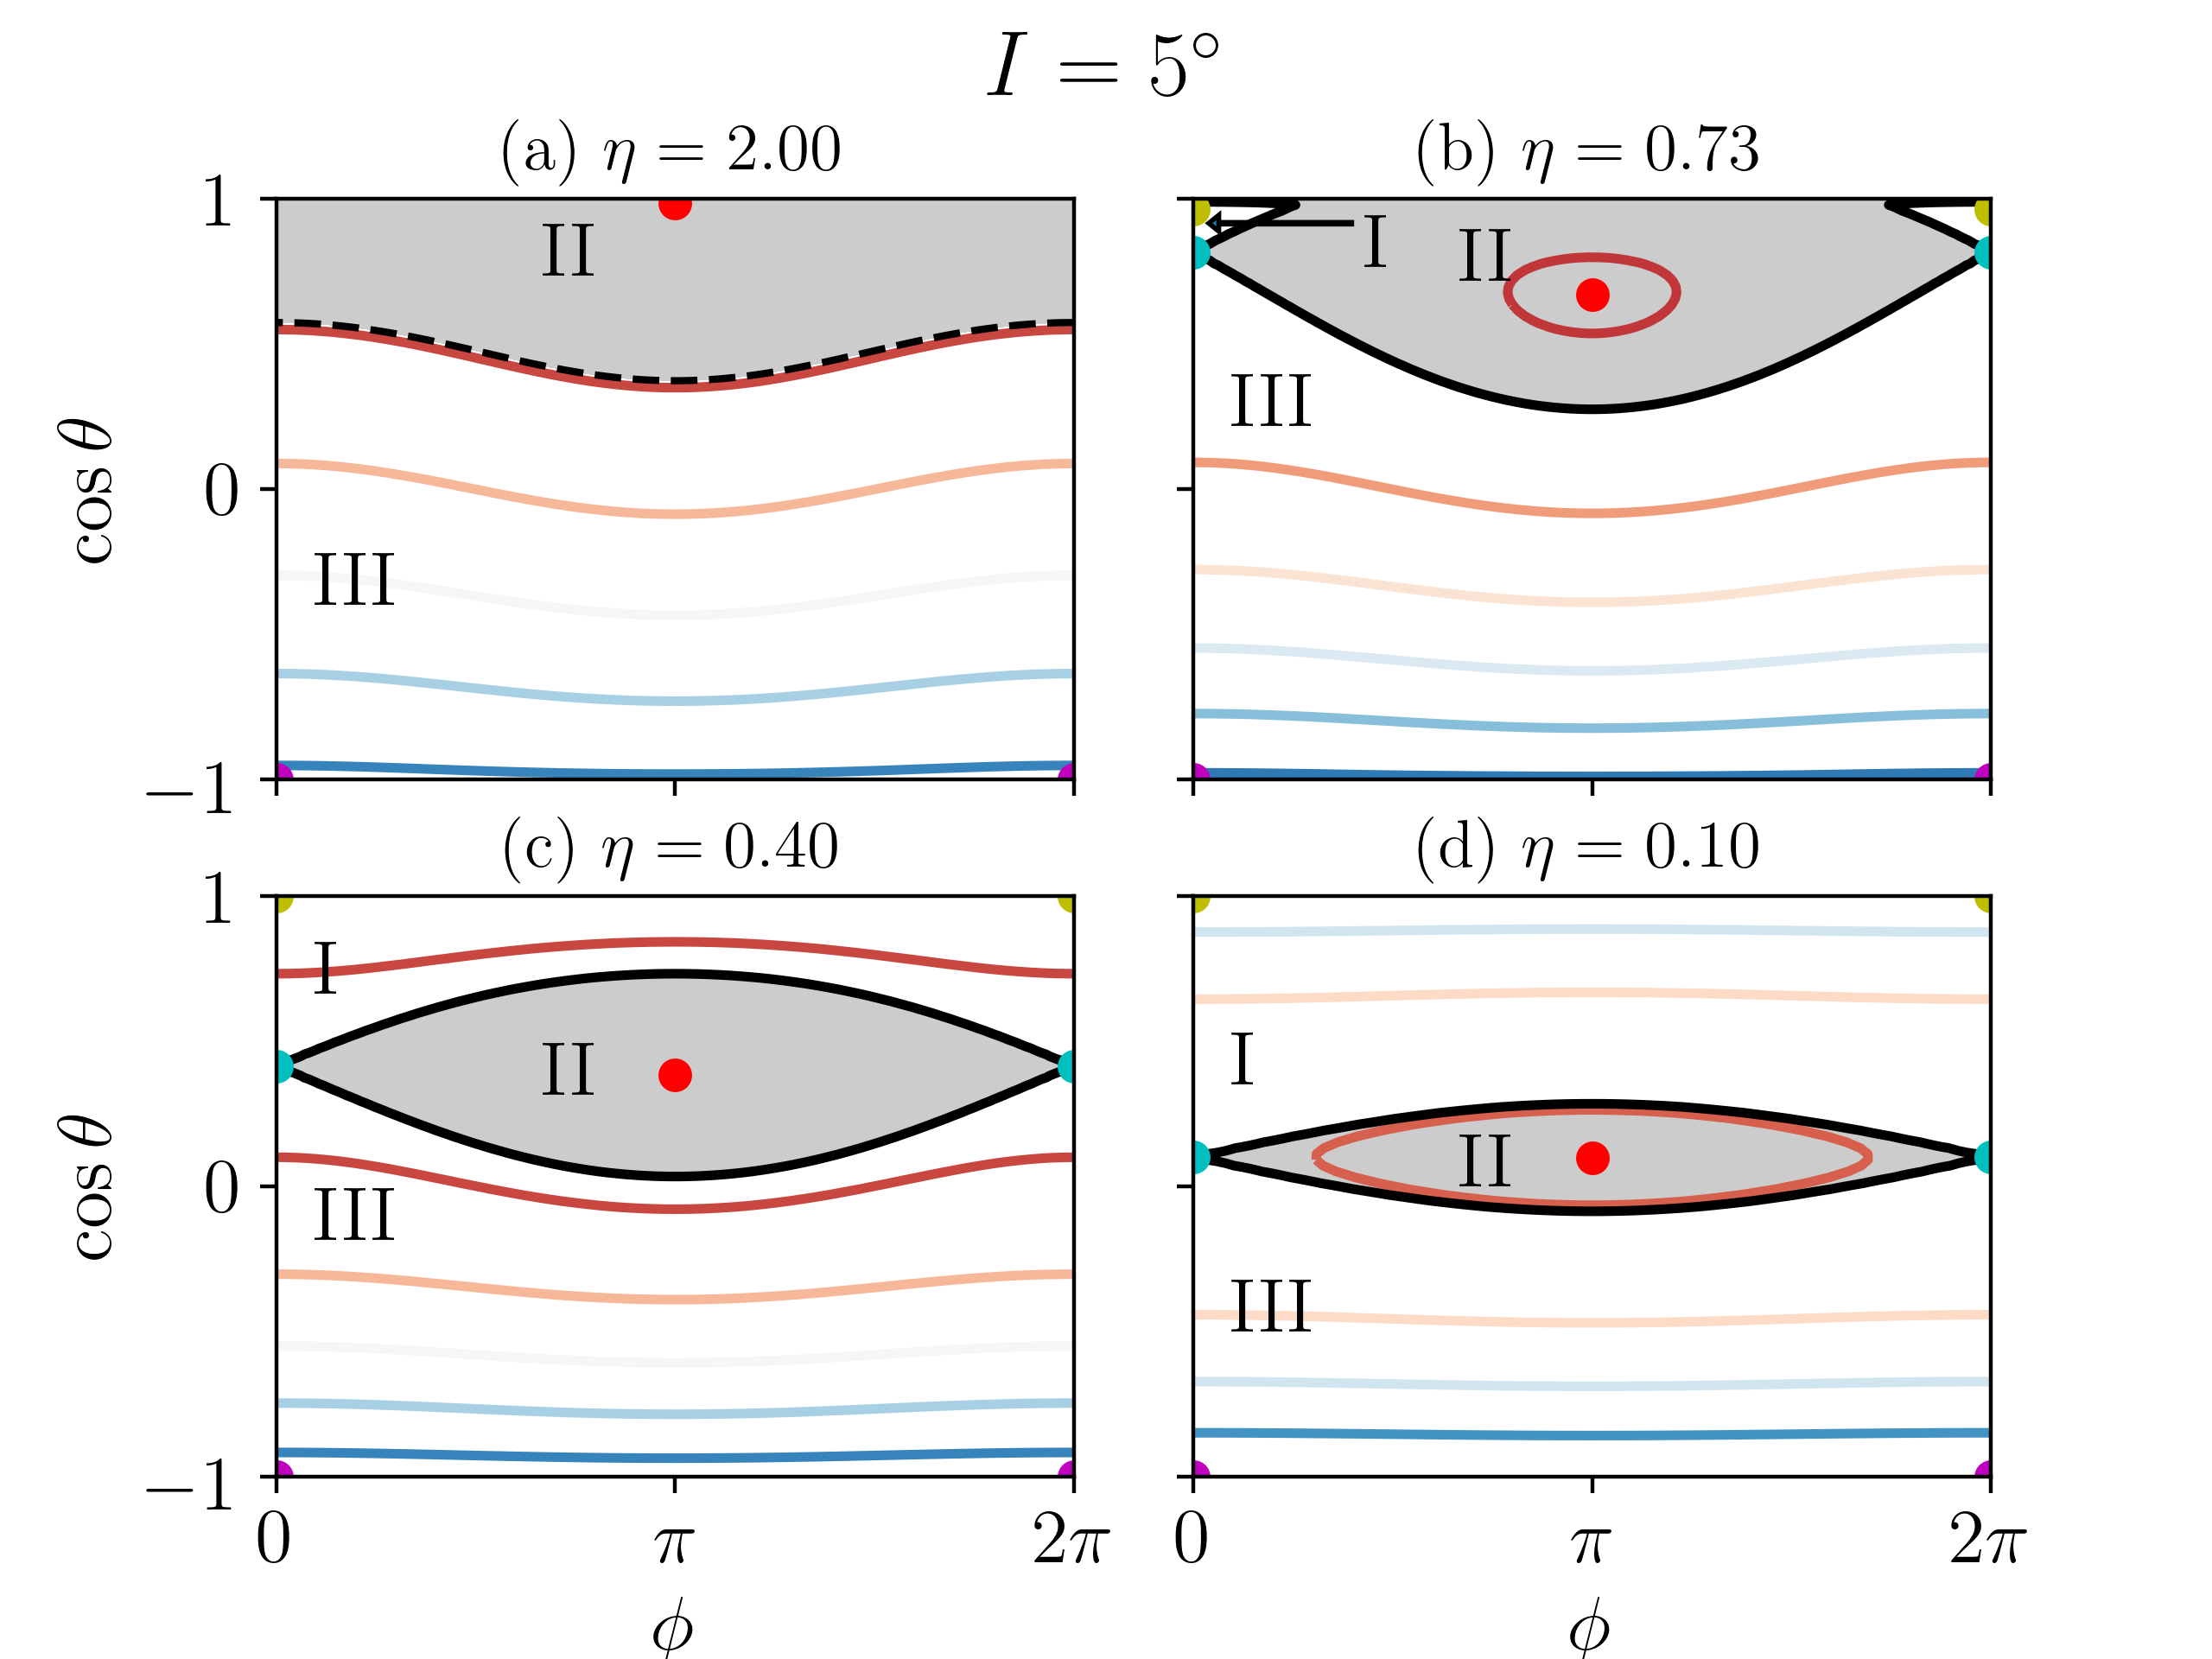
\includegraphics[width=\columnwidth]{../initial/0_eta/1contours_flip.png}
    \caption{Contour plot of $H\p{\phi, \cos \theta}$. Black dotted line is the
    separatrix, which only exists for $\eta < \eta_c$.}\label{fig:eq_1contours}
\end{figure}

The locations of the $\cos\theta$ of the two/four CSs as a function of $\eta$ is
provided in
\begin{figure}[t]
    \centering
    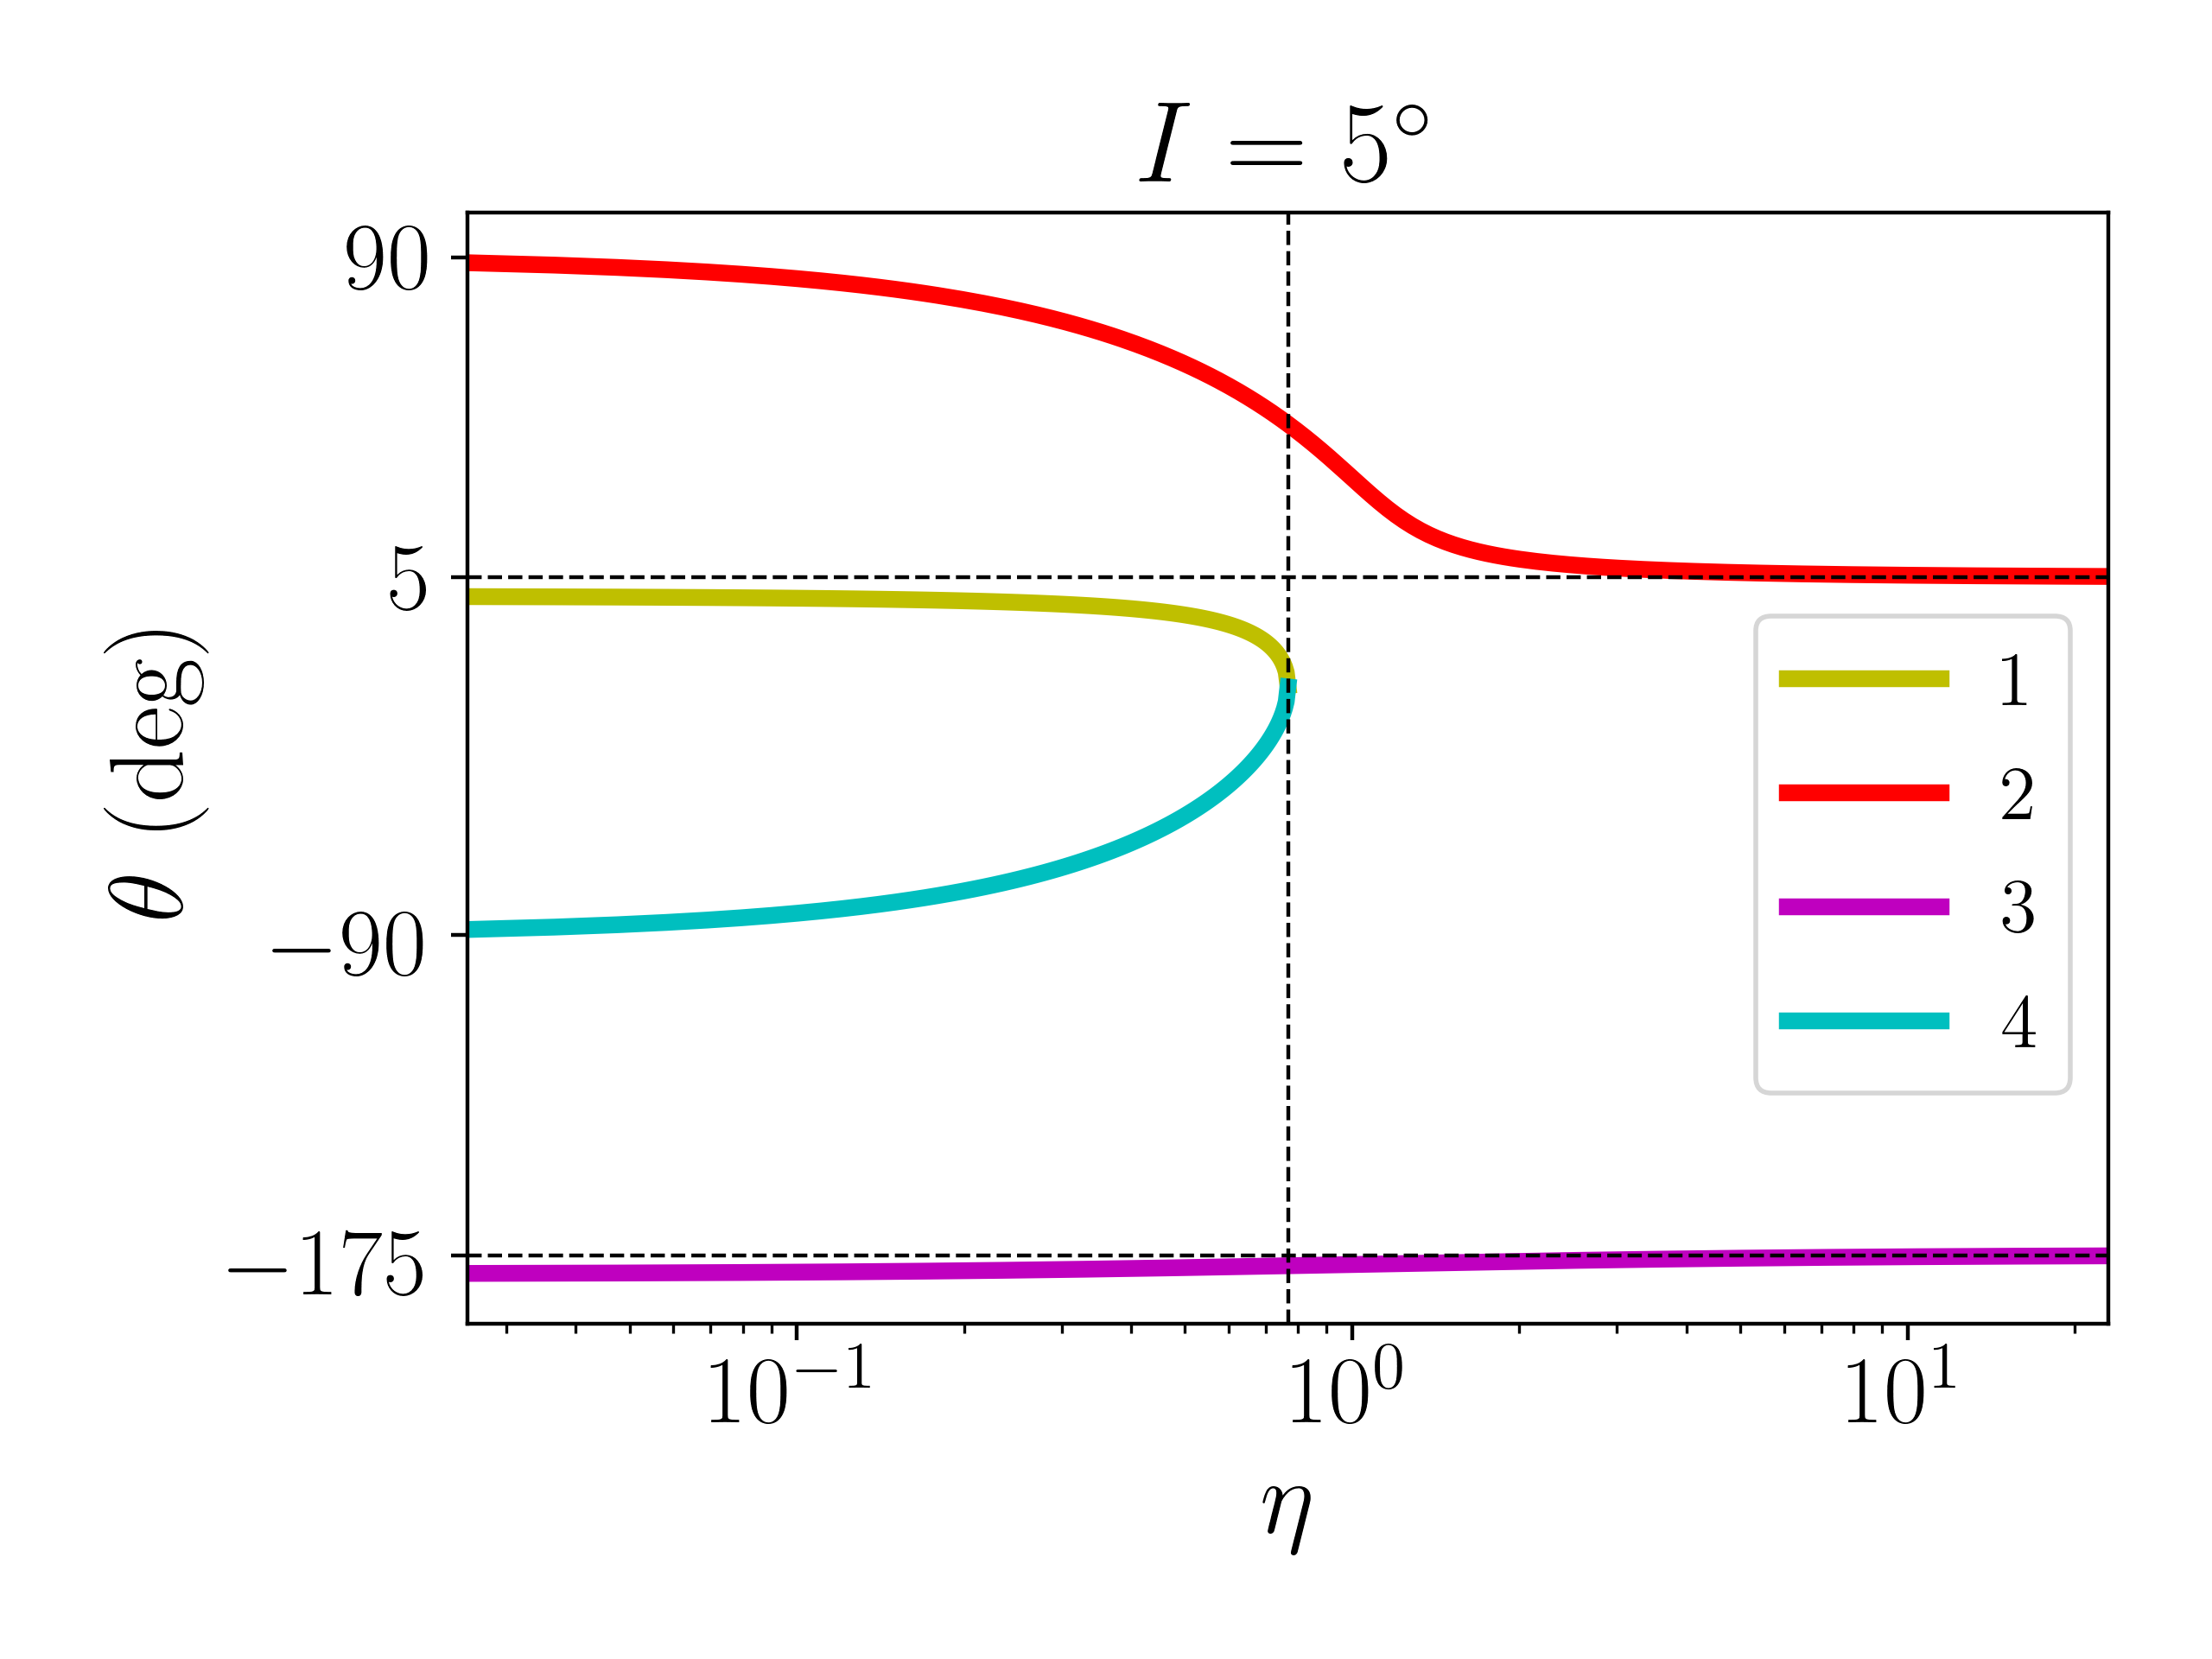
\includegraphics[width=\columnwidth]{../initial/99_misc/2_cs_locs.png}
    \caption{Locations of the Cassini states over time, following the same
    coloring scheme as \autoref{fig:eq_1contours}.}\label{fig:cs_locs}
\end{figure}

\subsection{Separatrix}

In the four-CS regime, one of the CSs is a saddle point, conventionally denoted
Cassini State 4 (CS4). All trajectories are periodic with finite period except
two critical trajectories asymptotic in the past and future to CS4. Together,
these two critical trajectories are referred to as the \emph{separatrix} and
divide phase space into three zones. We use notation described in
\autoref{fig:eq_1contours}.

The unsigned area enclosed by the separatrix is known exactly in literature
\citep{henrard1987,ward2004I}:
\begin{subequations}\label{se:area_ward}
    \begin{align}
        z_0 &= \eta\cos I,\nonumber\\
        \chi &= \sqrt{-\frac{\tan^3\theta_4}{\tan I} - 1},\nonumber\\
        \rho &= \chi \frac{\sin^2 \theta_4\cos \theta_4}{
            \chi^2 \cos^2\theta_4 + 1},\nonumber\\
        T &= 2\chi \frac{\cos \theta_4}{
            \chi^2 \cos^2\theta_4 - 1},\nonumber\\
        A_{II} &= 8\rho + 4\arctan T - 8z_0 \arctan \frac{1}{\chi},\\
        A_I &= 2\pi\p{1 - z_0} - \frac{A_2}{2},\\
        A_{III} &= 2\pi\p{1 + z_0} - \frac{A_2}{2}.
    \end{align}
\end{subequations}
These are plotted as a function of $\eta$ in \autoref{fig:eq_areas}.
\begin{figure}
    \centering
    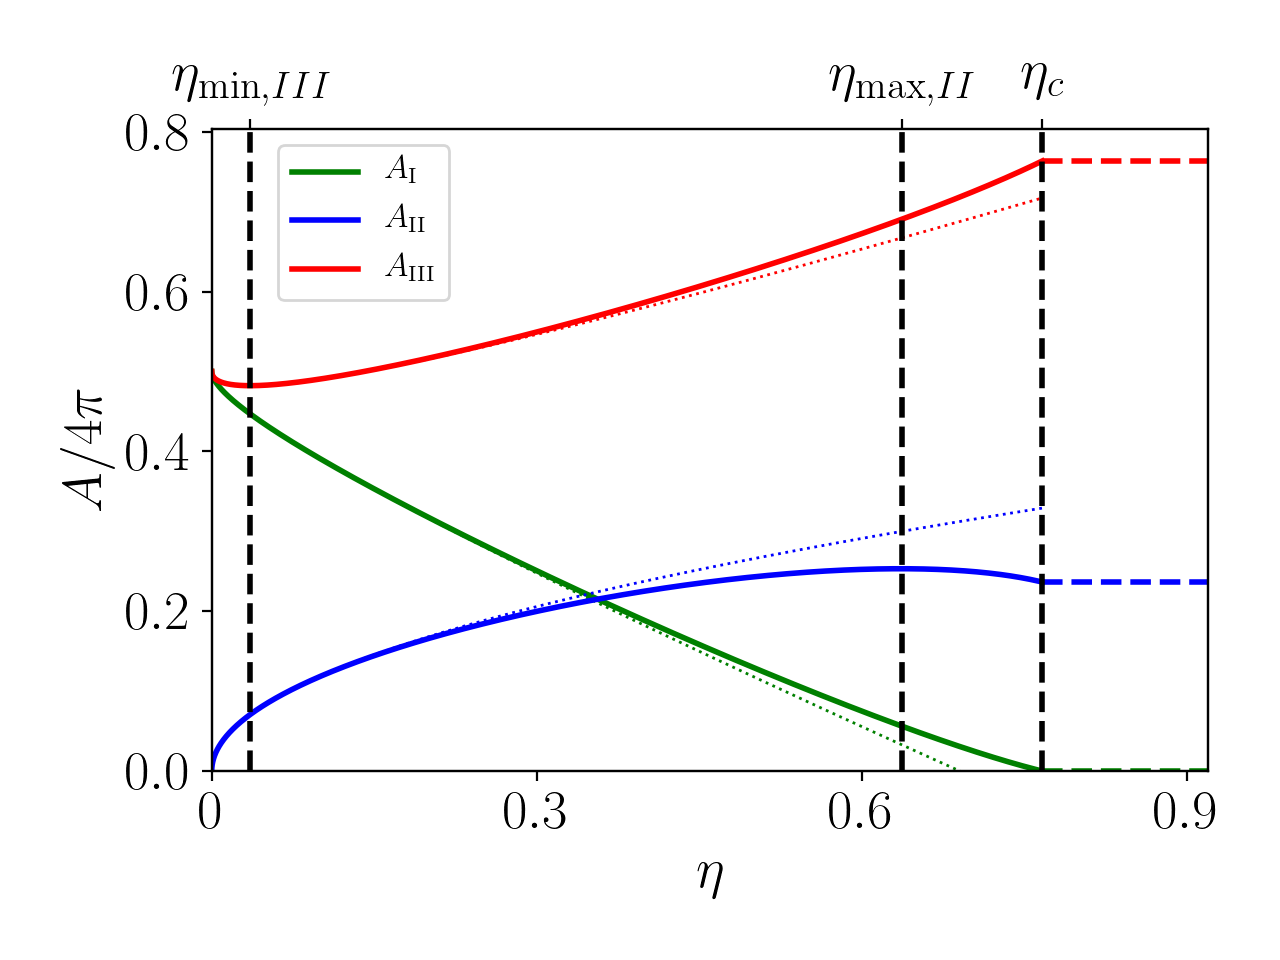
\includegraphics[width=\columnwidth]{../initial/99_misc/1_areas.png}
    \caption{Plot of $A_{i}(\eta)$ as given by \autoref{se:area_ward}. Dotted
    lines correspond to small $\eta$ approximations discussed in
    \autoref{ss:app_transition}.}\label{fig:eq_areas}
\end{figure}

\section{Adiabatic Evolution}\label{s:ad}

In the truly adiabatic limit, $\epsilon \to 0$; we use $\epsilon =
3 \times 10^{-4}$ in \autoref{ss:ad_fid} and vary $\epsilon$ in
\autoref{ss:ad_ensemble}. The adiabatic limit is quantified
in~\cite{millholland_disk} to be
\begin{equation}
    \dot{\eta} \lesssim \dots \label{eq:ad_constr}
\end{equation}

\subsection{Individual Simulations}\label{ss:ad_fid}

In the limit $\eta \to 0$, all trajectories circulate with constant
\begin{equation}
    \theta_{f} \equiv \s{\arccos \hat{s} \cdot \hat{l}}_{\eta \to 0}.
\end{equation}
We run simulations that terminate at $\eta = 10^{-5}$ and measure
$\theta_{f}$. We vary the initial
\begin{equation}
    \theta_{sd, i} \equiv \s{\arccos \hat{s} \cdot \hat{l}_d}_{t=0}.
\end{equation}

Initially, in the $\eta > \eta_c$ regime, only zones $II, III$ exist.
Conversely, at the end of the simulation when $\eta \to 0$, only zones $I, III$
exist. Naively then, one might expect four sequences of transitions
between zones (``zone transition histories'') to appear during simulations: (i)
$II \to I$, (ii) $II \to III$, (iii) $III \to I$, and (iv) the trivial $III \to
III$ where the trajectory never encounters the separatrix. In fact, (v) a fifth
possible history involving two transitions is observed $III \to II \to I$.

Between zone transitions, the adiabatic invariant $J \equiv \oint \cos\theta
\;\mathrm{d}\phi$ is conserved. Here, we adopt convention $J$ is a \emph{signed}
area
\begin{equation}
    J = \oint \p{1 - \cos \theta}\;\mathrm{d}\phi.
\end{equation}
This has the advantage of (i) having a removable singularity when the trajectory
crosses $\cos \theta = 1$, and (ii) being easily expressible as combinations of
the $A_i$ of \autoref{se:area_ward} without $2\pi$ offsets.

Given this definition, the change in $J$ during a separatrix encounter is easily
understood \citep{henrard1982}. We present in \autoref{fig:ad_21} a fiducial
simulaiton undergoing the $II \to I$ zone transition. An initial condition in
zone II with initial adiabatic invariant $J_i > 0$ librates about CS2 until
$A_{II} = J_i$. At this point, it encounters the separatrix and moves into zone I
with $J_f = -A_I$. Further simulations illustrating the other zone transition
histories are depicted in \autoref{s:app_histories}.
\begin{figure}
    \centering
    \begin{subfigure}{\columnwidth}
        \centering
        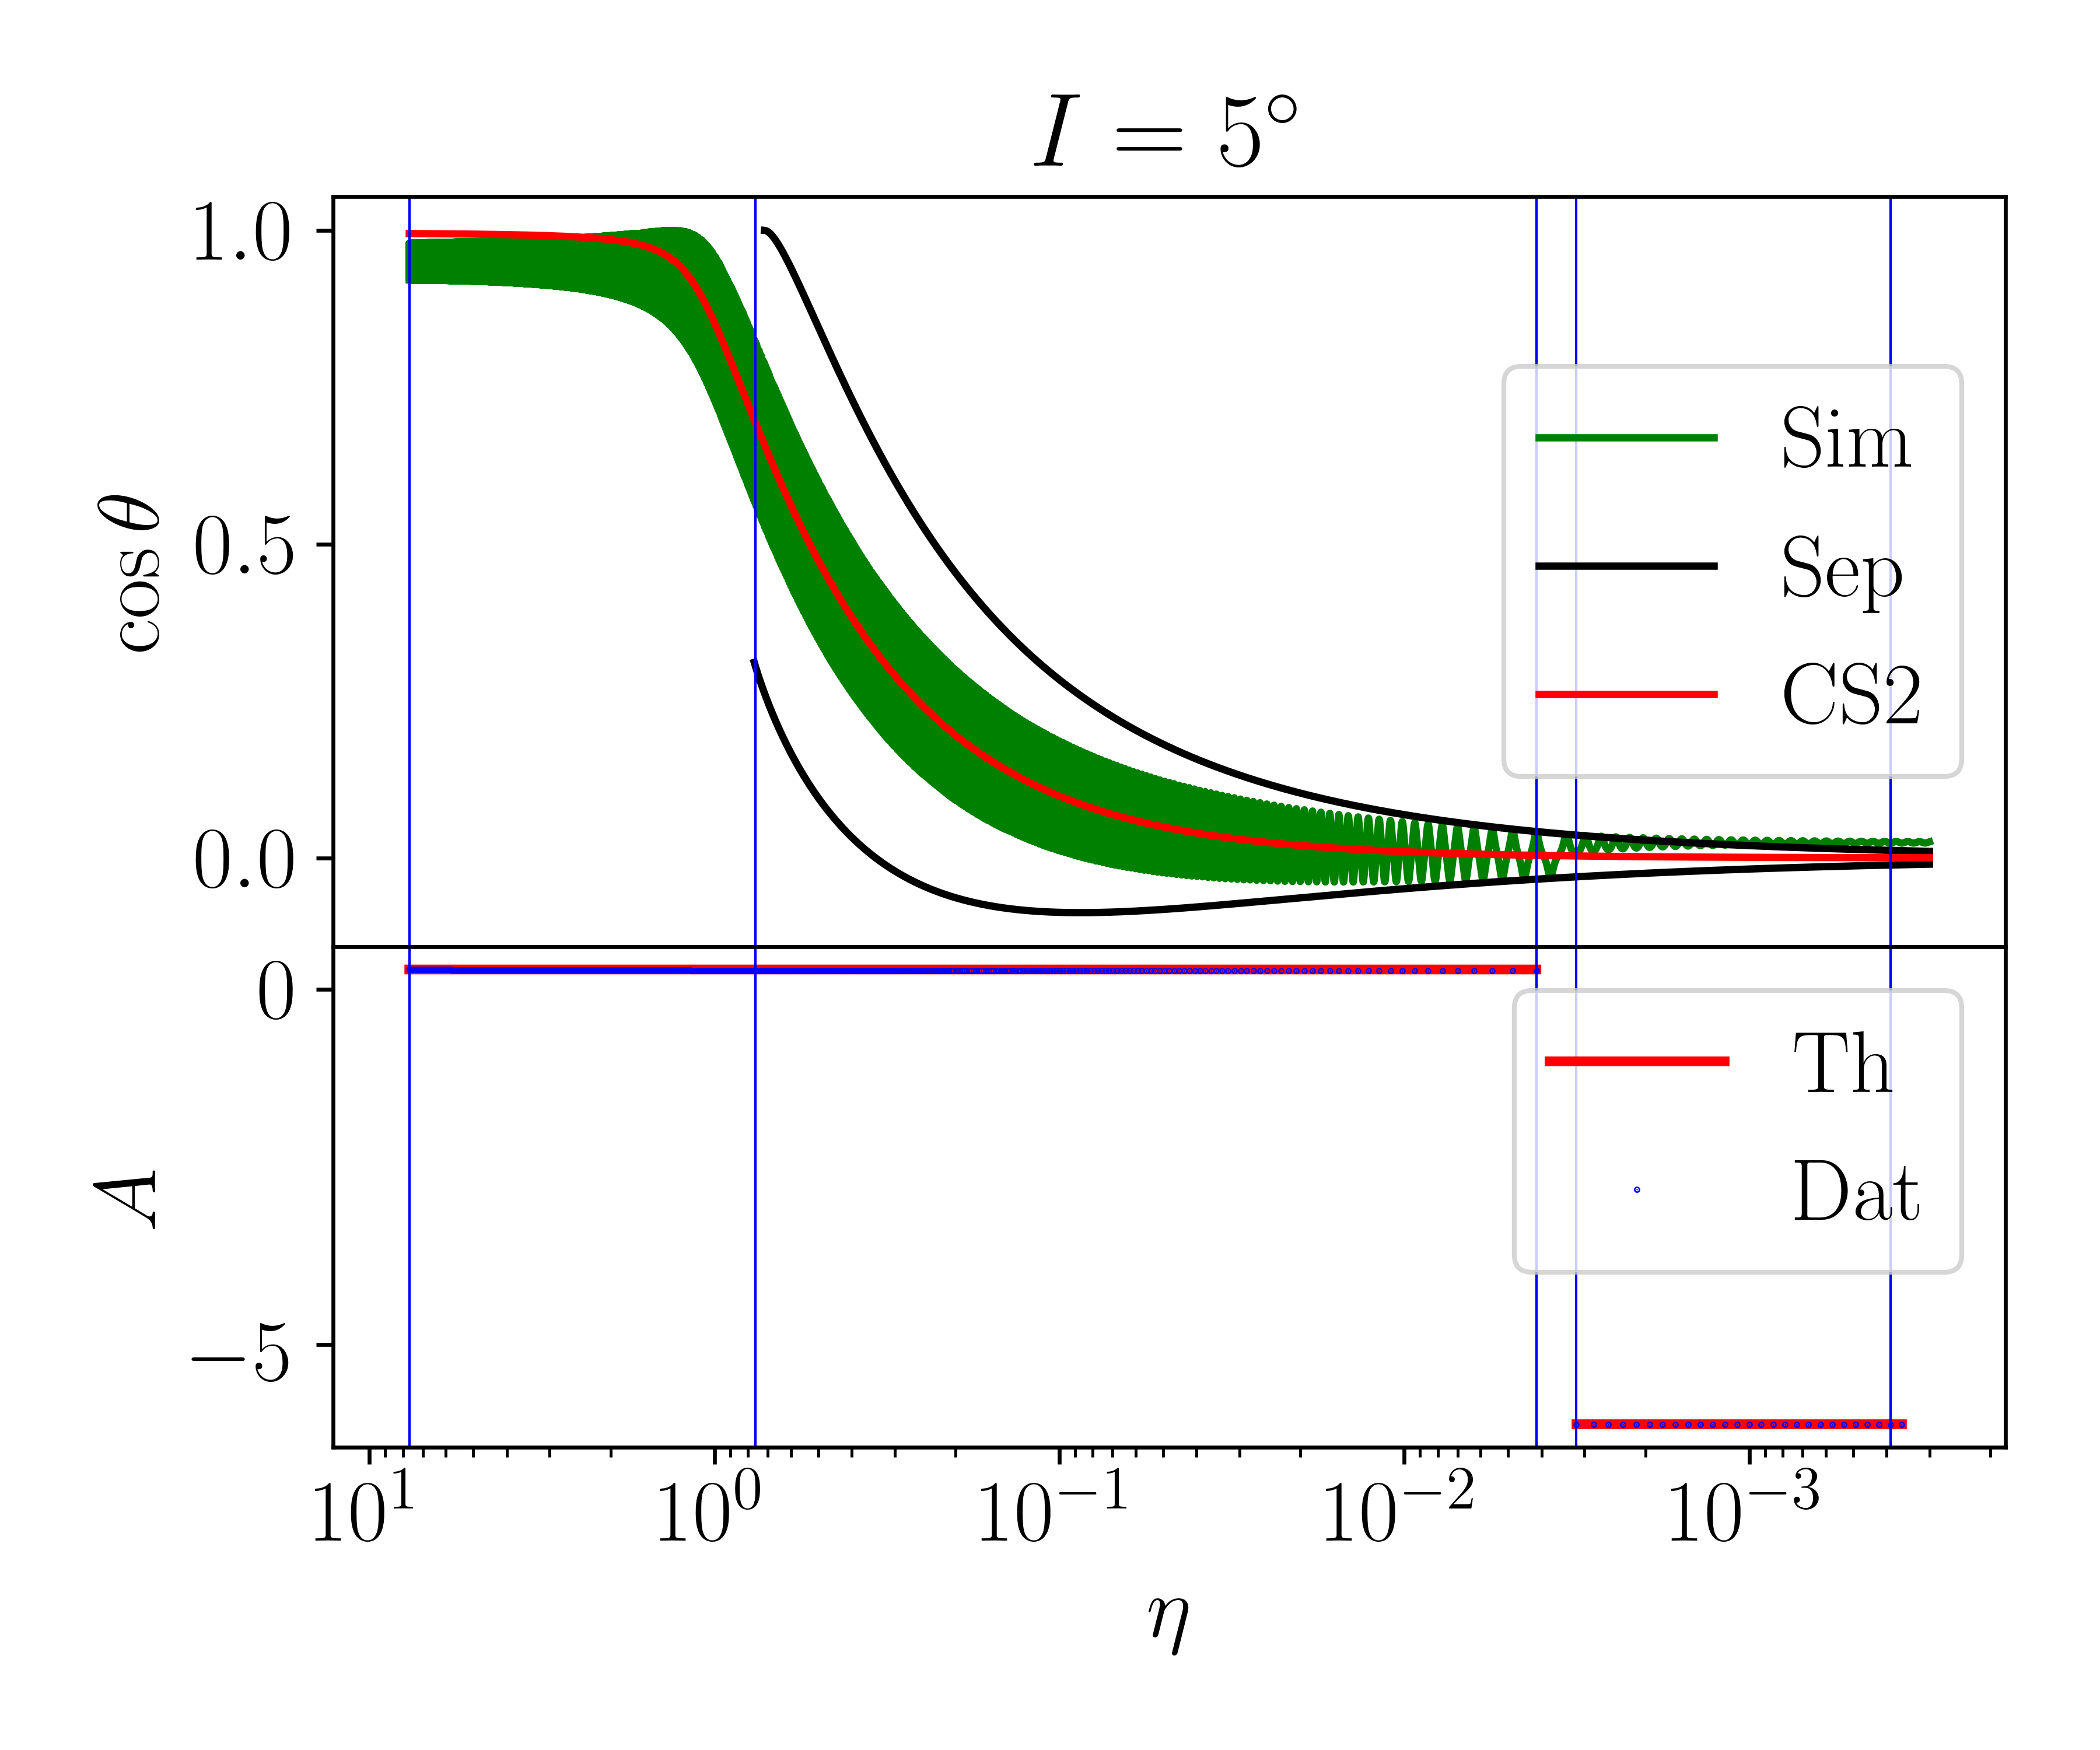
\includegraphics[width=\columnwidth]{../initial/2_toy2/3testo21.png}
        \caption{Top: Plot of $\cos \theta(t)$ (grey) over an example
        simulation. Overlaid are the locations of Cassini State 2 (blue), upper
        and lower bounds on the separatrix (dashed green), and value of
        $\theta_{f}$ predicted in the adiabatic limit (horizontal red line).
        Bottom: Plot of the enclosed separatrix area obtained by integrating the
        simulated trajectory (blue dots) and fully adiabitic theory (red line).
        A small blip in the data area arises when the integration area crosses
        the coordinate singularity at the pole. Vertical red magenta lines
        denote the four snapshots depicted below; they correspond to the start
        of the simulation, the appearance of the separatrix, the separatrix
        encounter and the end of the simulation.}
    \end{subfigure}
    \begin{subfigure}{\columnwidth}
        \centering
        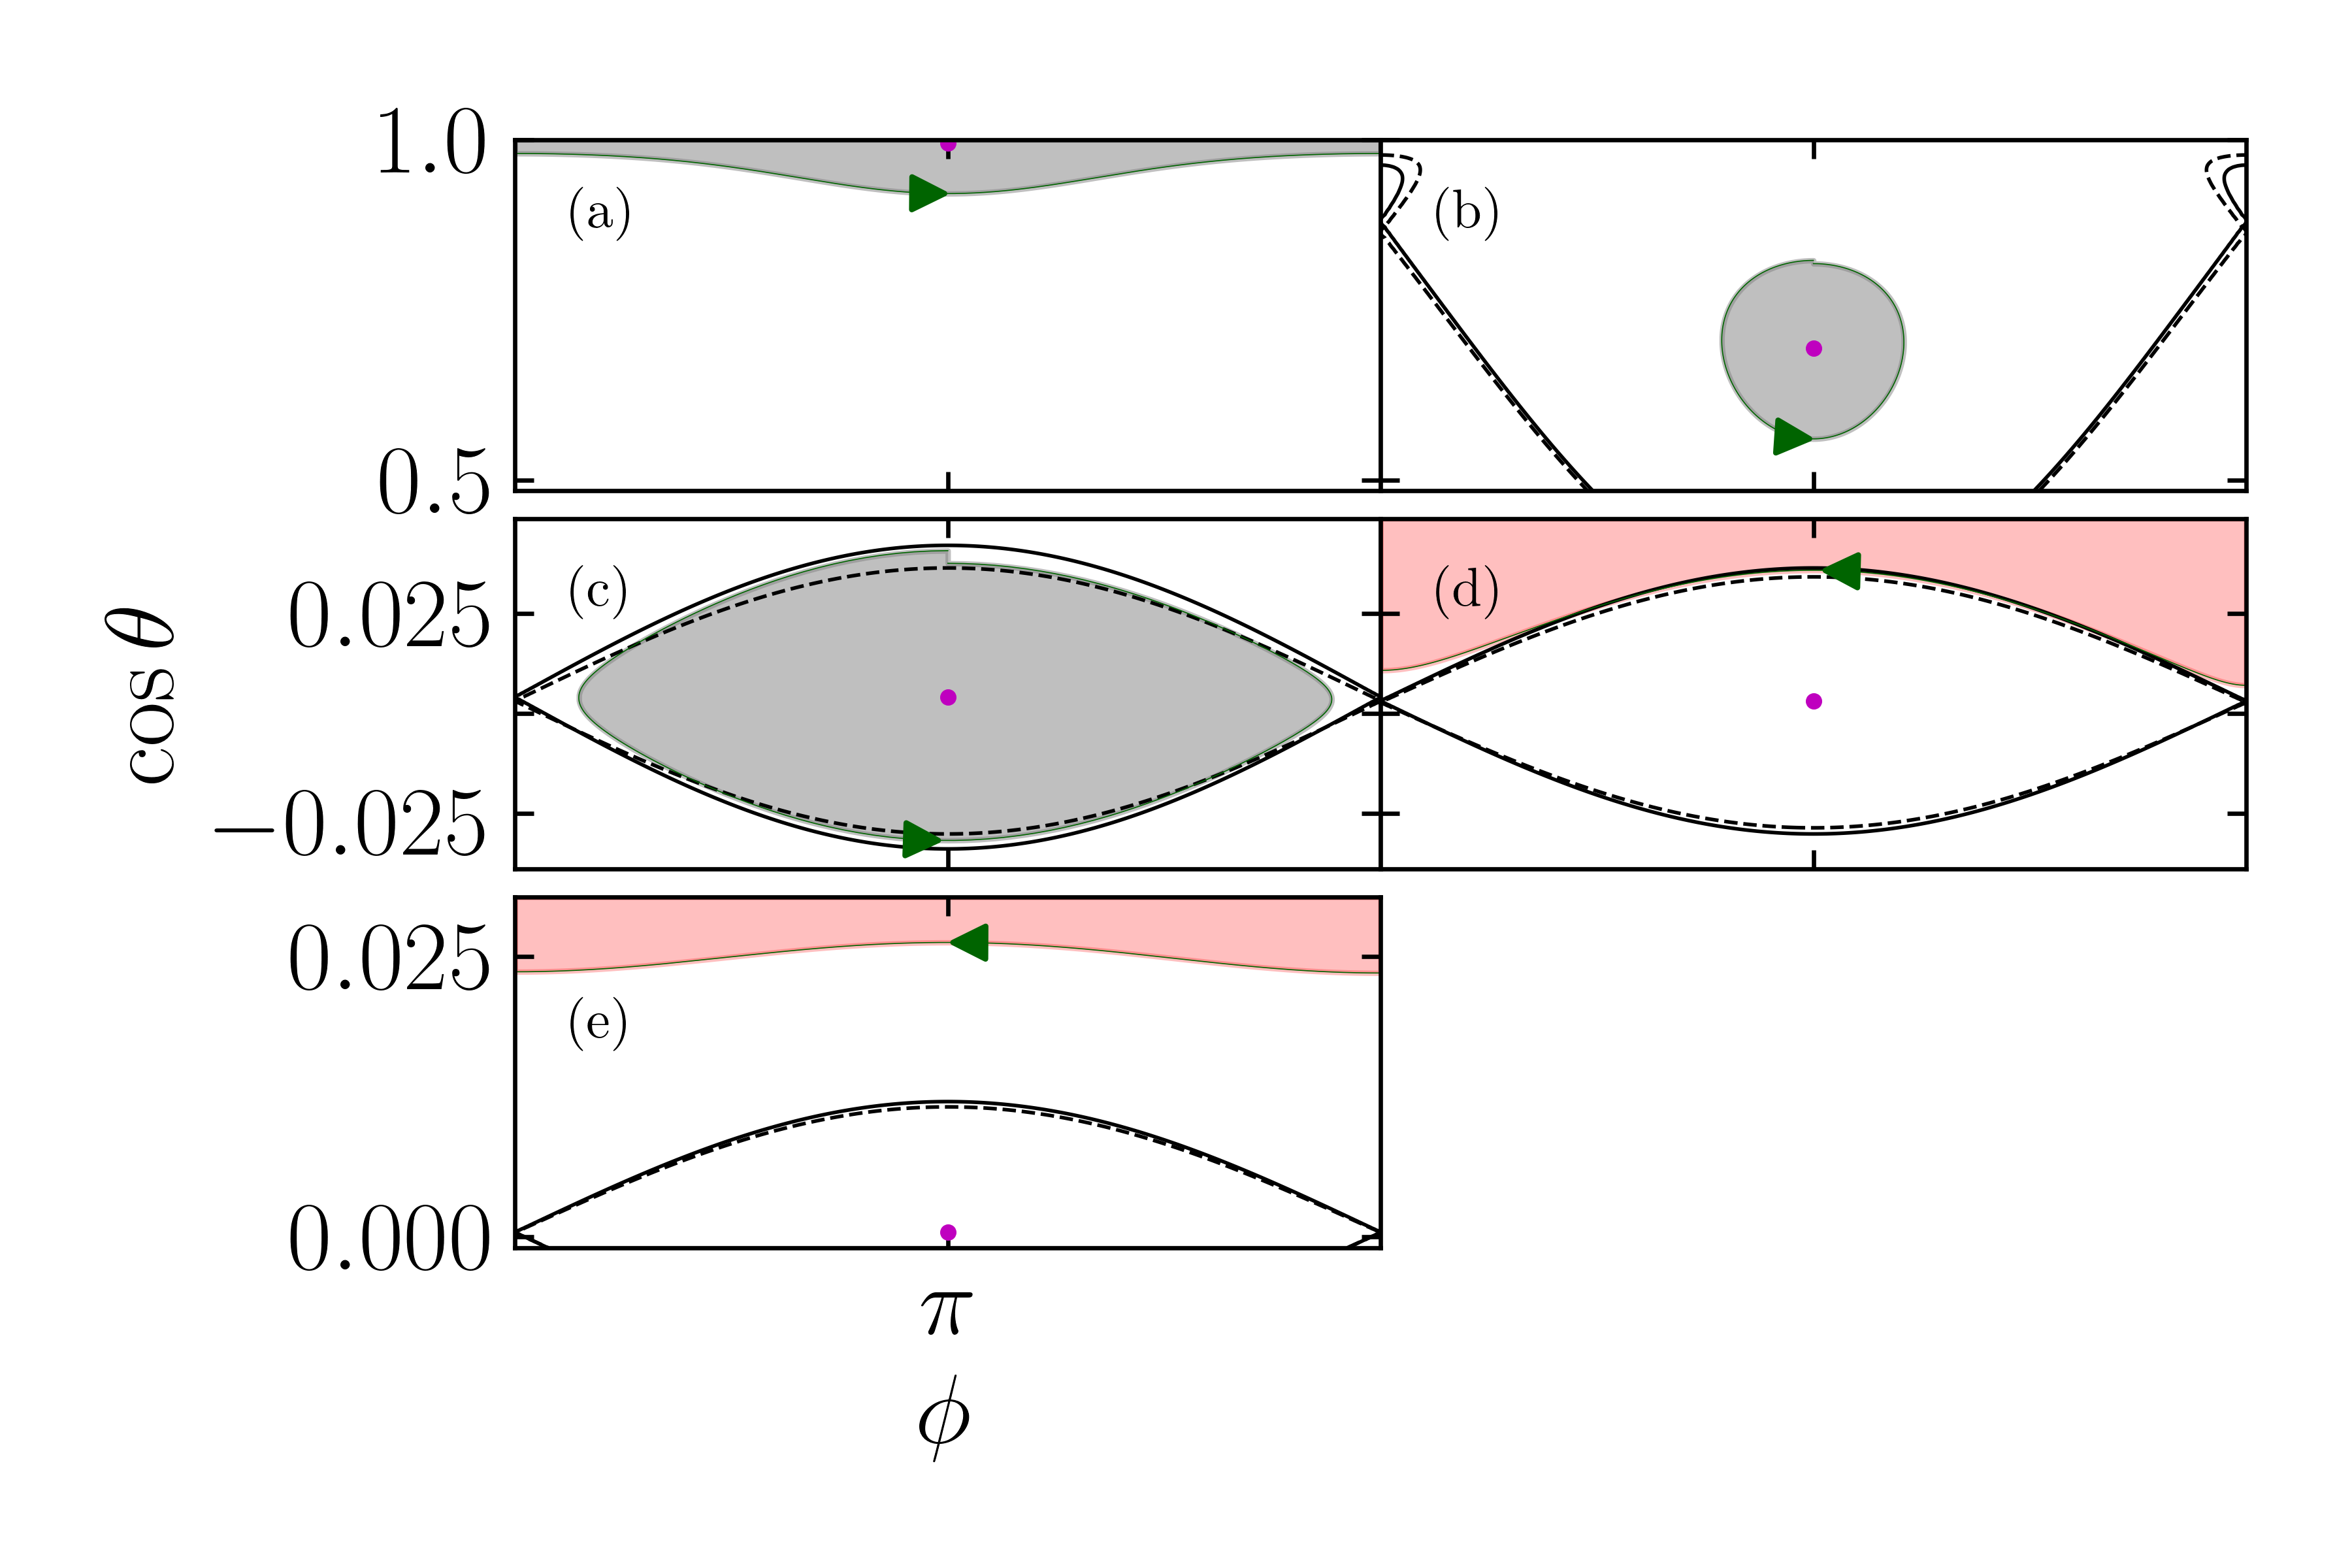
\includegraphics[width=\columnwidth]{../initial/2_toy2/3testo21_subplots.png}
        \caption{Snapshots in the $\p{\cos \theta, \phi}$ space of the
        simulation trajectories for two circulation/libration cycles around the
        $\eta$ values depicted above. Cycles are defined by the range of
        integration used to compute enclosed phase space area. Black dots denote
        the cycle immediately before the selected $\eta$ value, magenta dots the
        cycle immediately after, and grey denotes intermediate points that do
        not constitute a full cycle. Also labeled are the separatrix (green) and
        Cassini State 2 (blue).}
    \end{subfigure}
    \caption{Fiducial simulation following the $A_2 \to A_1$
    transition.}\label{fig:ad_21}
\end{figure}

\subsection{Dynamical Outcomes}\label{ss:ad_ensemble}

In the adiabatic limit, while separatrix encounters induce discontinuous changes
in enclosed phase space, the outcomes of these encounters are well understood in
pioneering work by Henrard \citep{henrard1982,henrard1987}. For a wide range of
$\theta_{sd, i}$, we run simulations over a ring of initial conditions at each
$\theta_{sd, i}$ and measure the final $\theta_{ f}$ values. We can also
predict the values of $\theta_{ f}$ for each of the dynamical histories as
well as their associated probabilities; refer to \autoref{ss:app_transition} for
details.
\begin{figure}
    \centering
    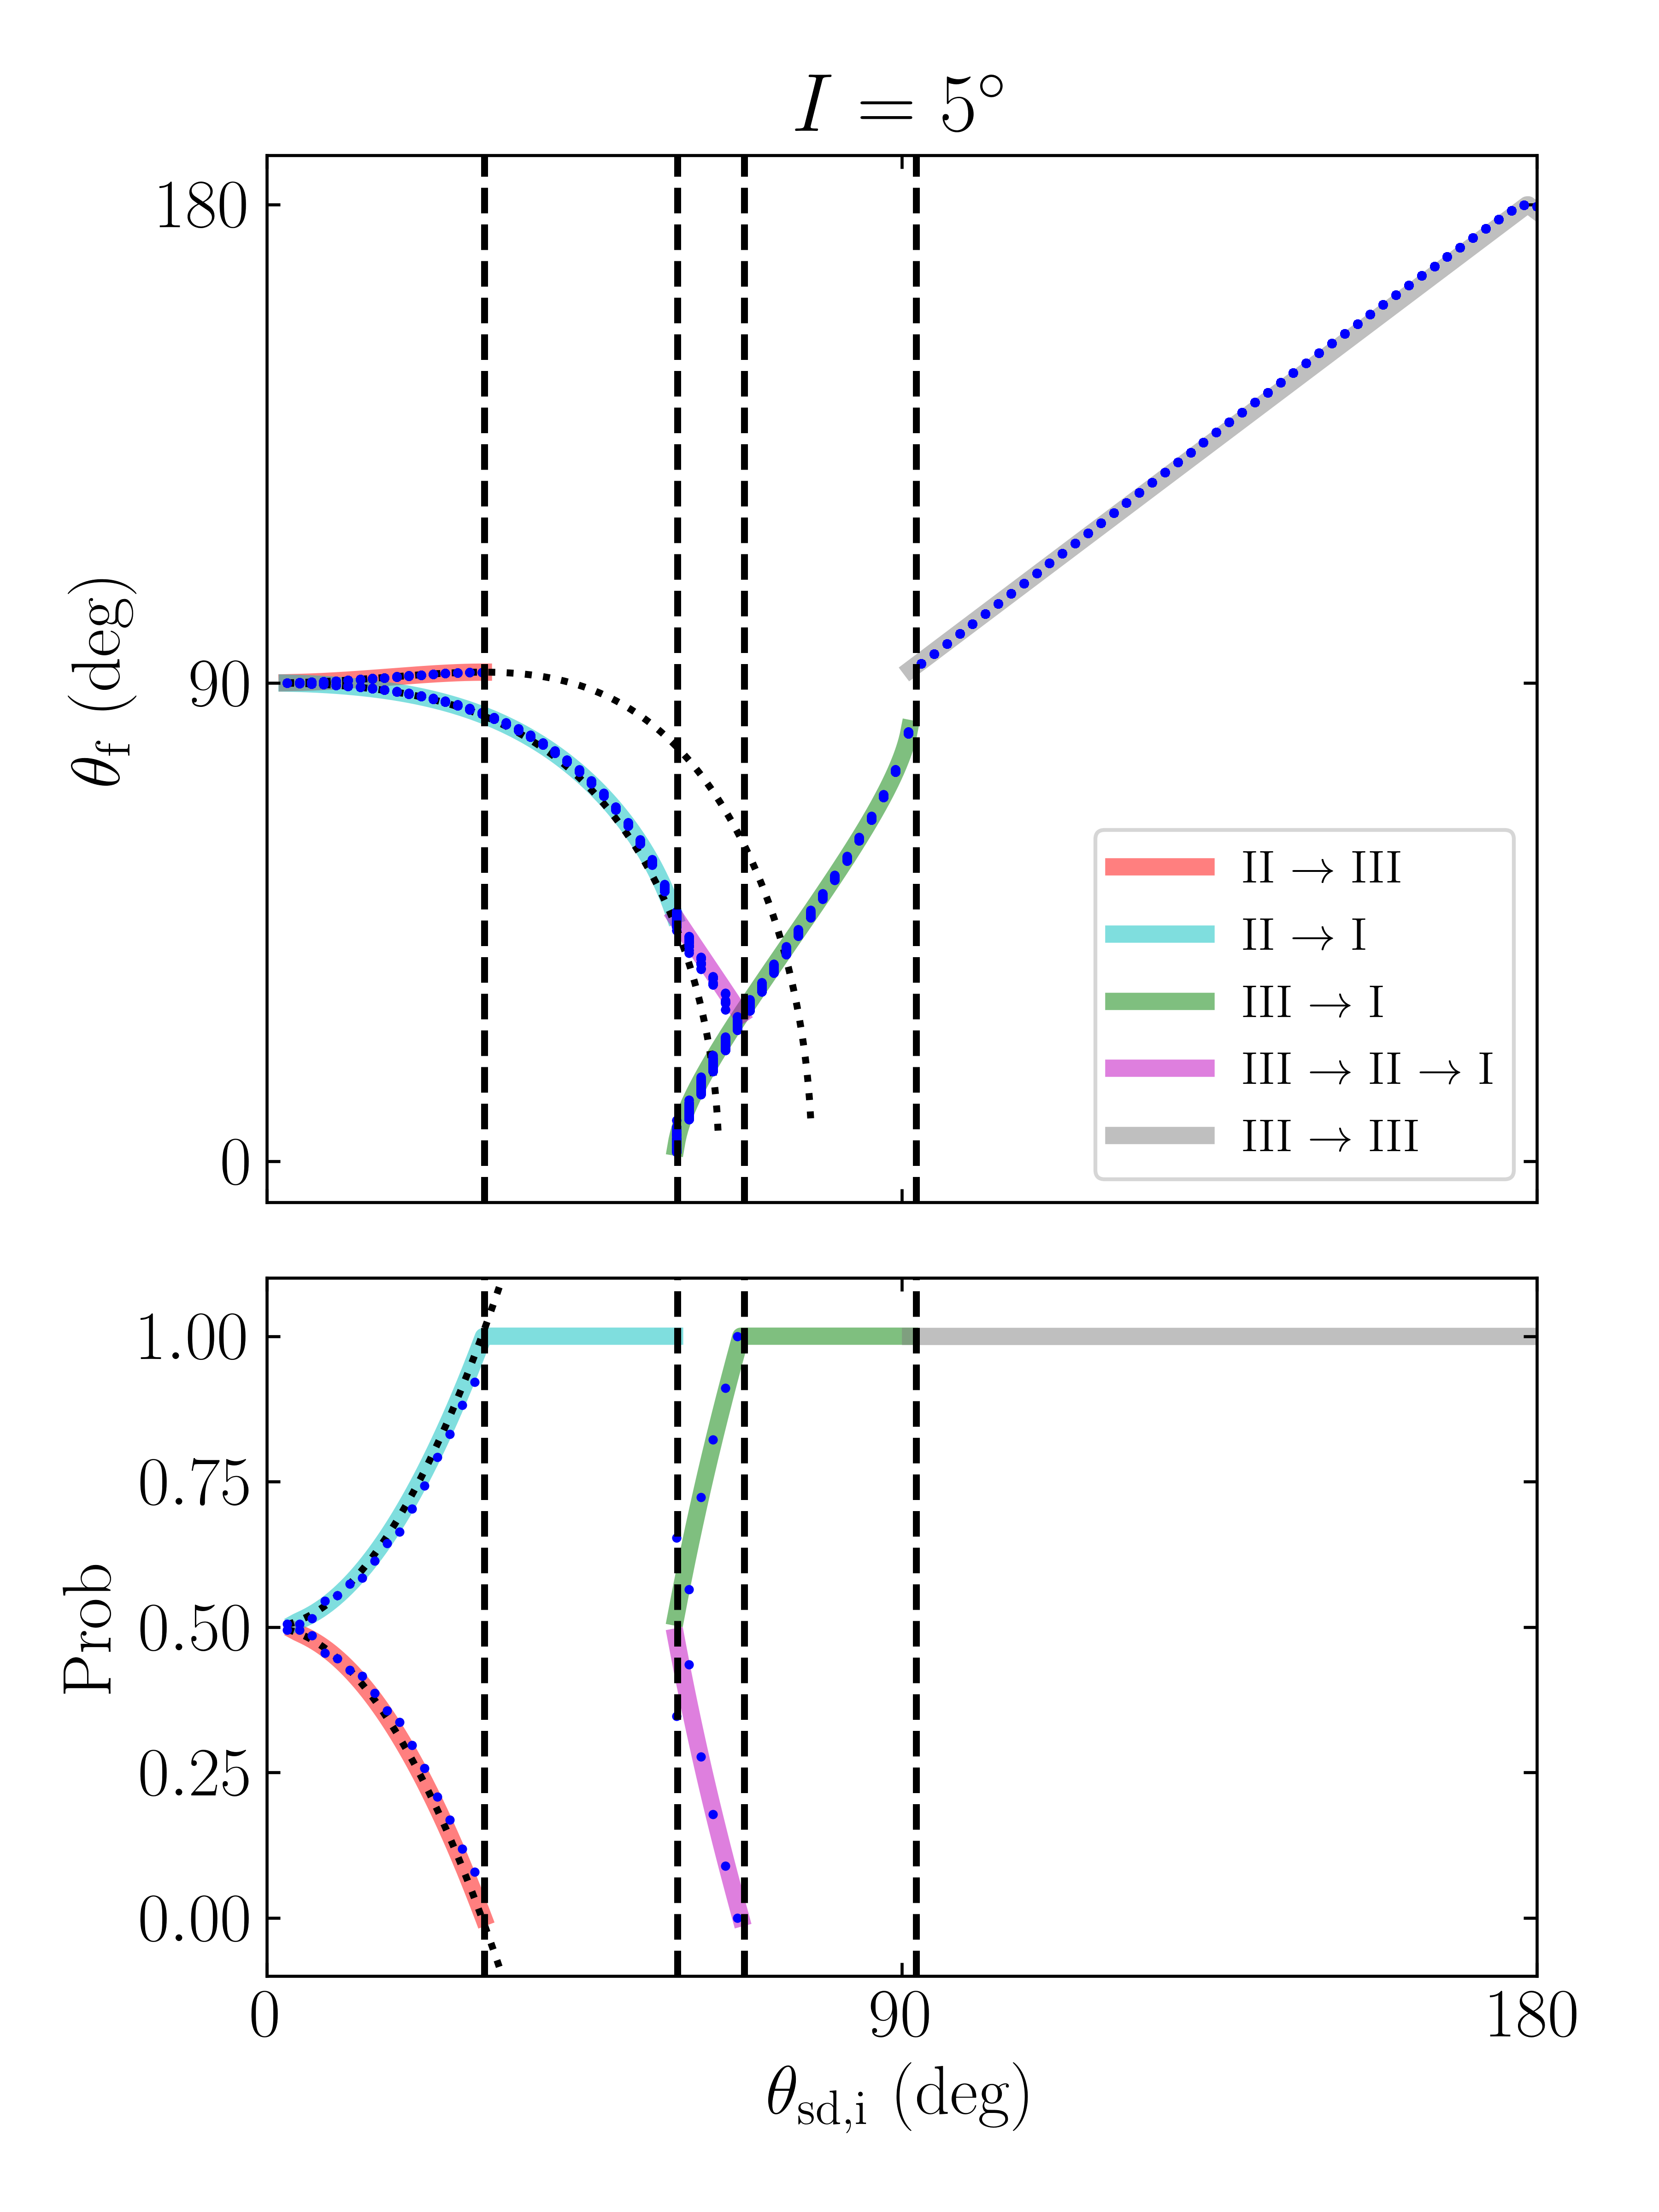
\includegraphics[width=\columnwidth]{../initial/2_toy2/3_ensemble_05_35.png}
    \caption{Top: $\theta_{f}\p{\theta_{sd, i}}$, overlaid with semi-analytic
    predictions of the $\theta_{ f}$ for each of the four nontrivial
    dynamical histories in colored lines. Bottom: Semi-analytic probabilities of
    each of the dynamical histories for each $\theta_{sd,
    i}$.}\label{fig:ad_ensemble}
\end{figure}

\section{Nonadiabatic Evolution}\label{s:nonad}

Here, we consider $\epsilon$ sufficiently large to violate the adiabiticity
constraint \autoref{eq:ad_constr}.

\subsection{Sample Trajectory}

A sample trajectory following in the style of \autoref{fig:ad_21} but for
$\epsilon = 0.1$ is provided in \autoref{fig:nonad_traj}.
\begin{figure}
    \centering
    \begin{subfigure}{\columnwidth}
        \centering
        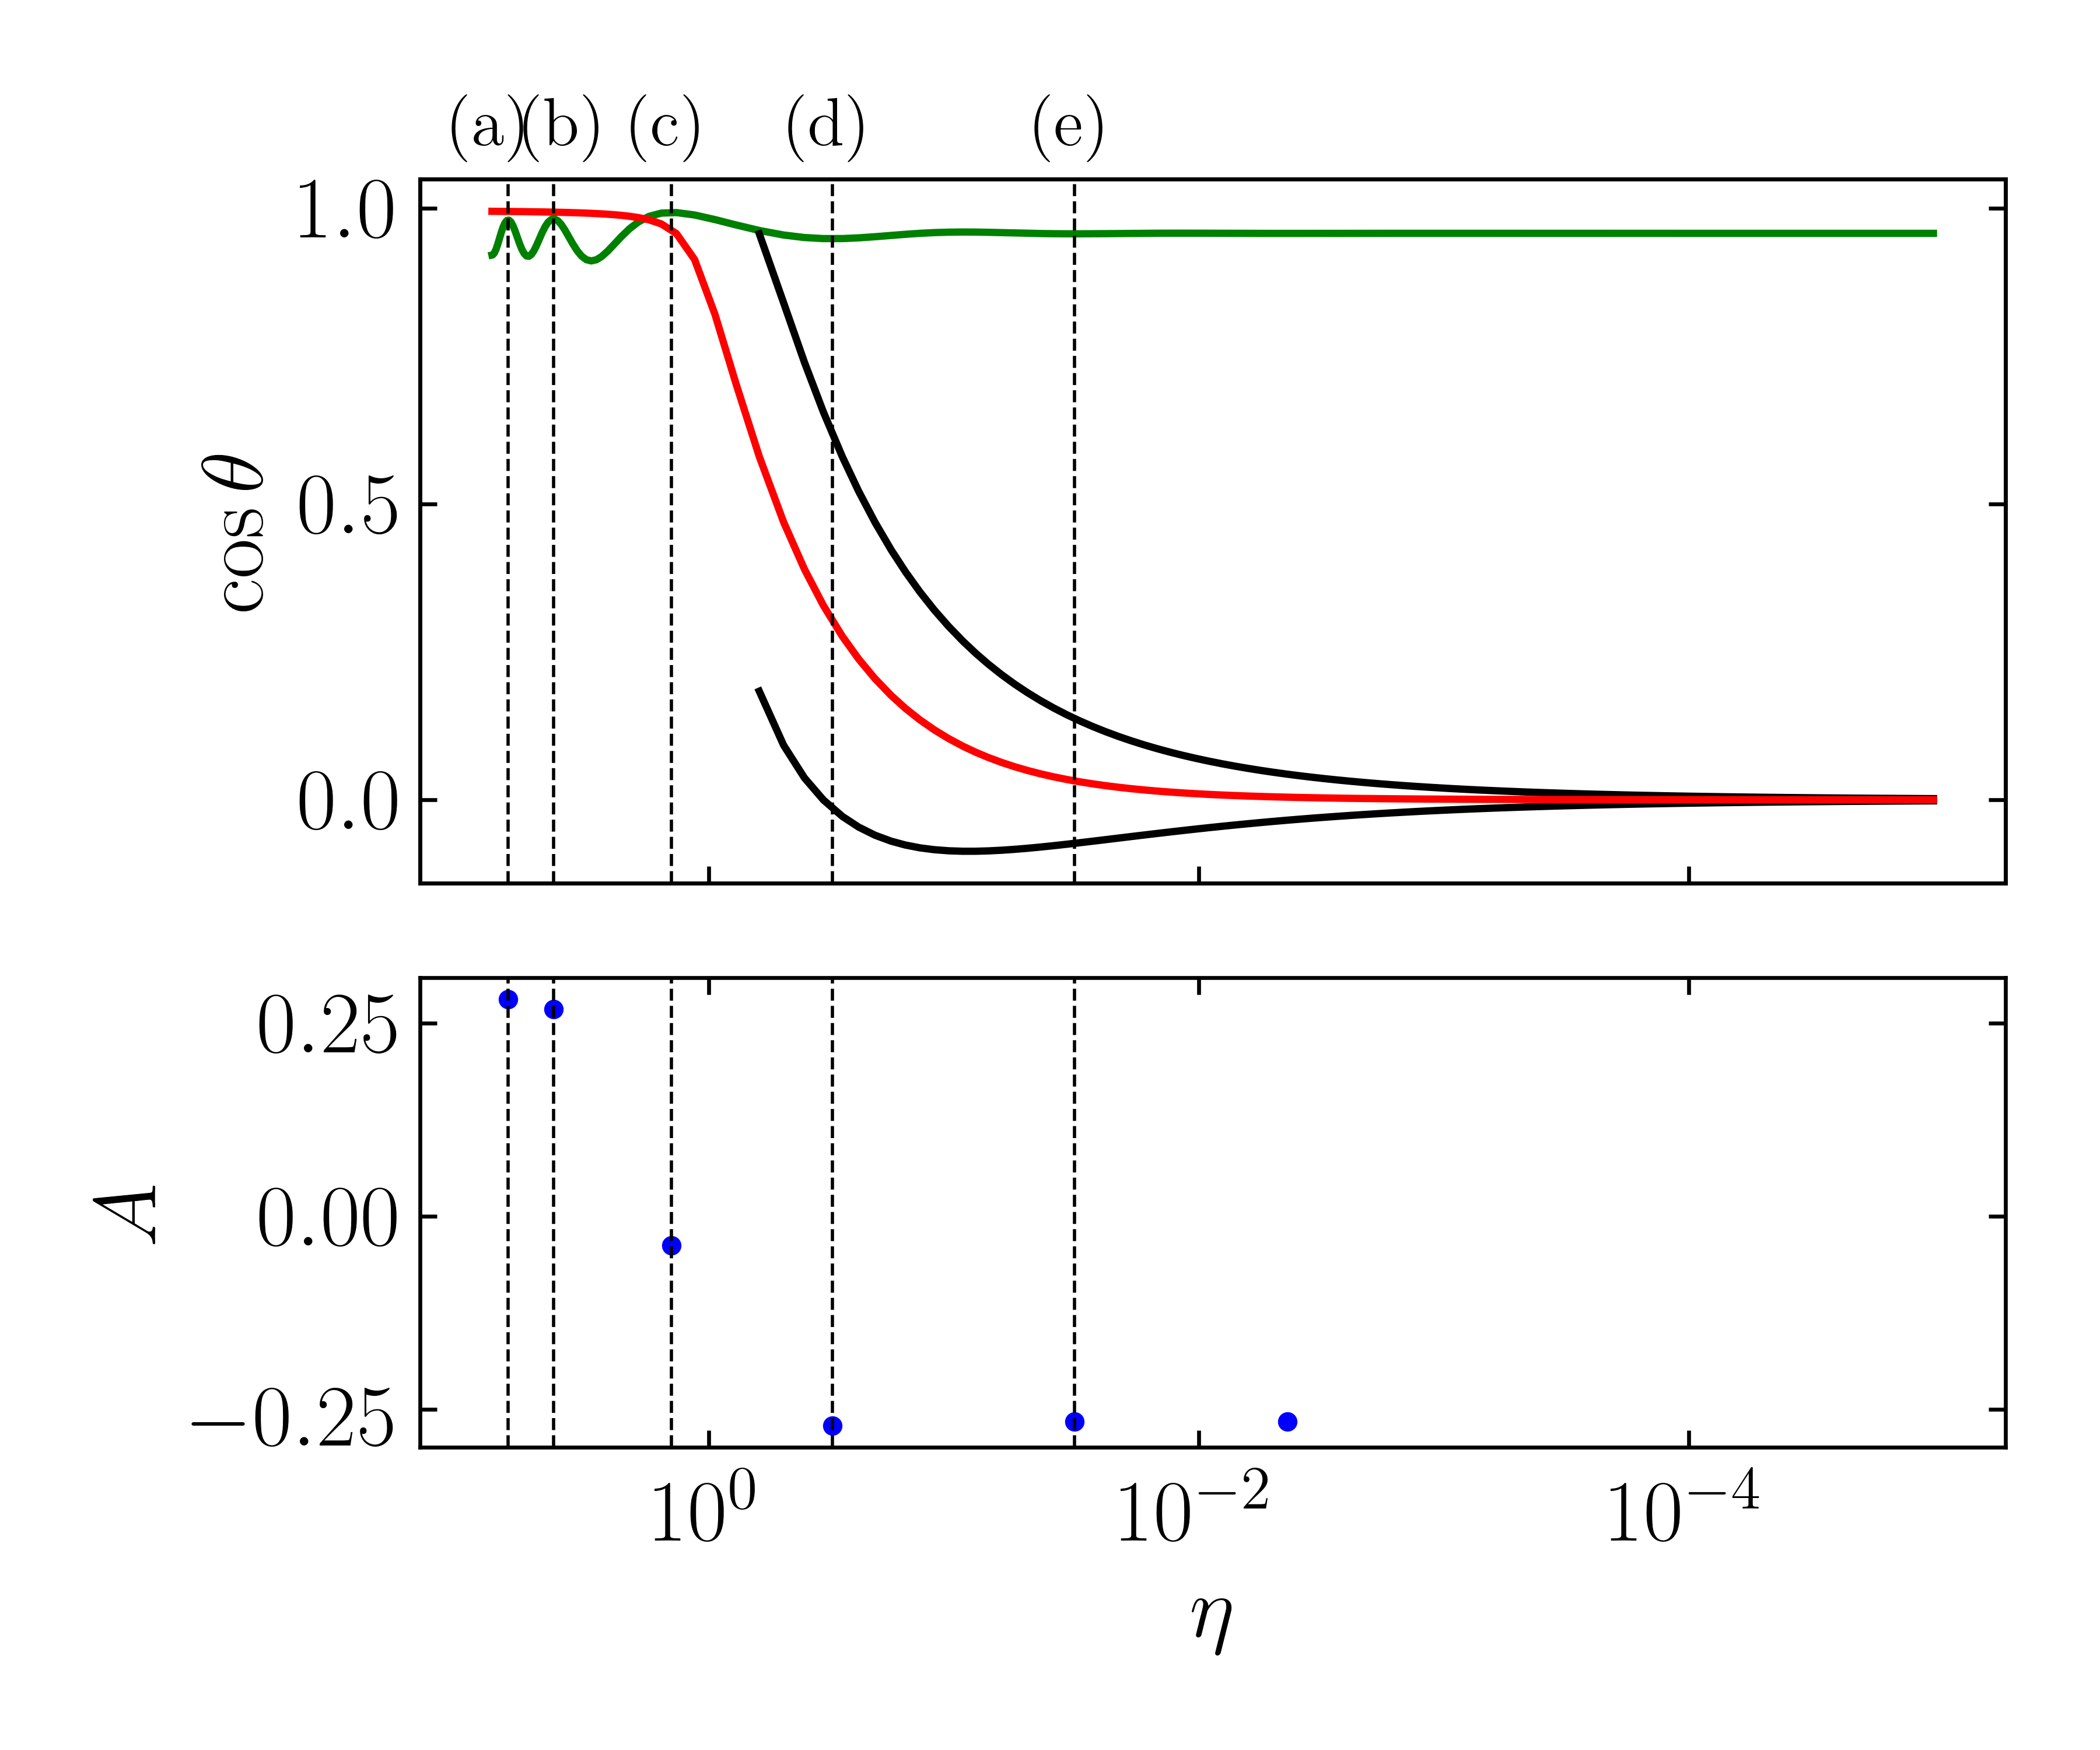
\includegraphics[width=\columnwidth]{../initial/2_toy2/3testo_nonad.png}
    \end{subfigure}
    \begin{subfigure}{\columnwidth}
        \centering
        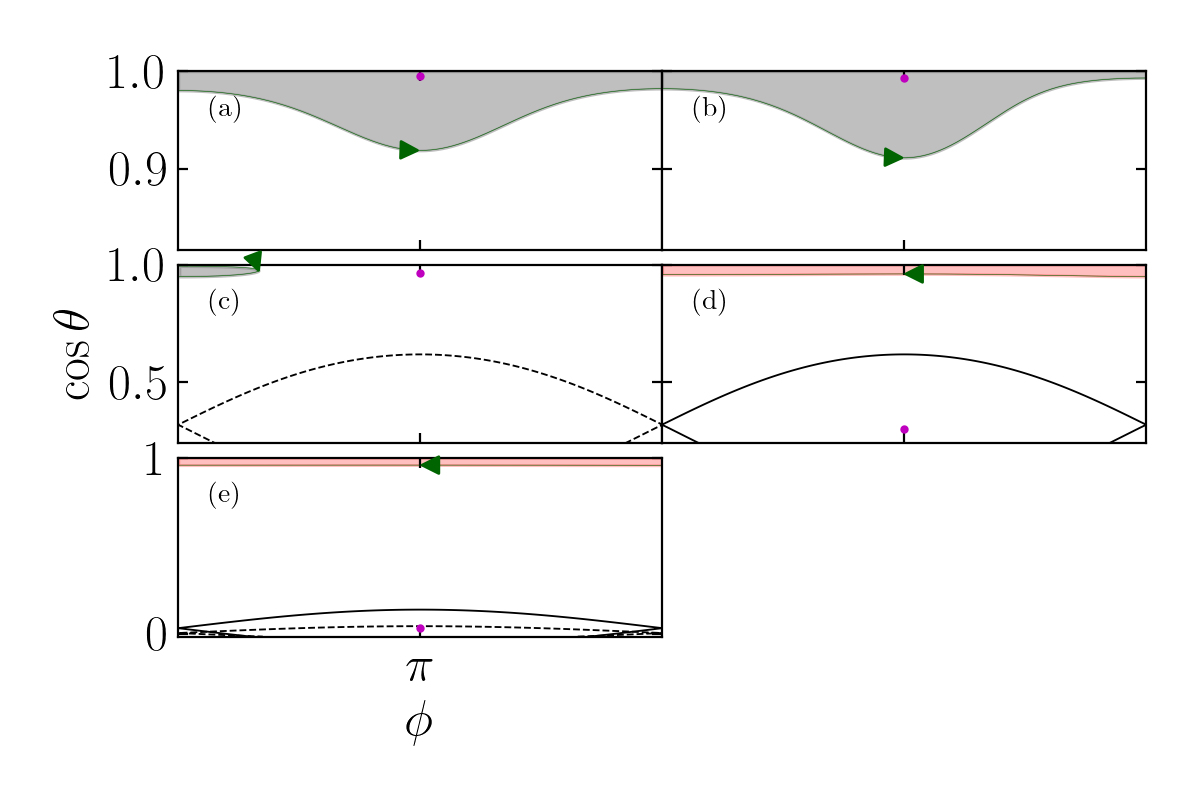
\includegraphics[width=\columnwidth]{../initial/2_toy2/3testo_nonad_subplots.png}
    \end{subfigure}
    \caption{Same as \autoref{fig:nonad_traj} but for a non-adiabatic $\epsilon =
    0.1$.}\label{fig:nonad_traj}
\end{figure}

\subsection{Dynamical Outcomes}

A formula for $\theta_{f}$ assuming $\theta_{sd, i} = 0$ initially can be
given:
\begin{equation}
    \theta_{f}\p{\theta_{sd, i} = 0} = \sqrt{\frac{2\pi \Omega}{\epsilon}}
        \tan I.\label{eq:nonad_q_f}
\end{equation}
We can naively generalize this by recognizing that any nonzero $\theta_{sd, i}$
manifests as obliquity variations as $\hat{s}$ librates about $\hat{l}_d$, and
these oscillations are ``frozen in'' when the disk dissipates. Thus,
\begin{equation}
    \theta_{f}\p{\theta_{sd, i}} \in \sqrt{\frac{2\pi \Omega}{\epsilon}}
        \tan I \pm \theta_{sd, i}.\label{eq:nonad_q_f_dist}
\end{equation}

We present the results of simulations for using $\epsilon = 0.3$ in
\autoref{fig:nonad_3_ensemeble}.
\begin{figure}
    \centering
    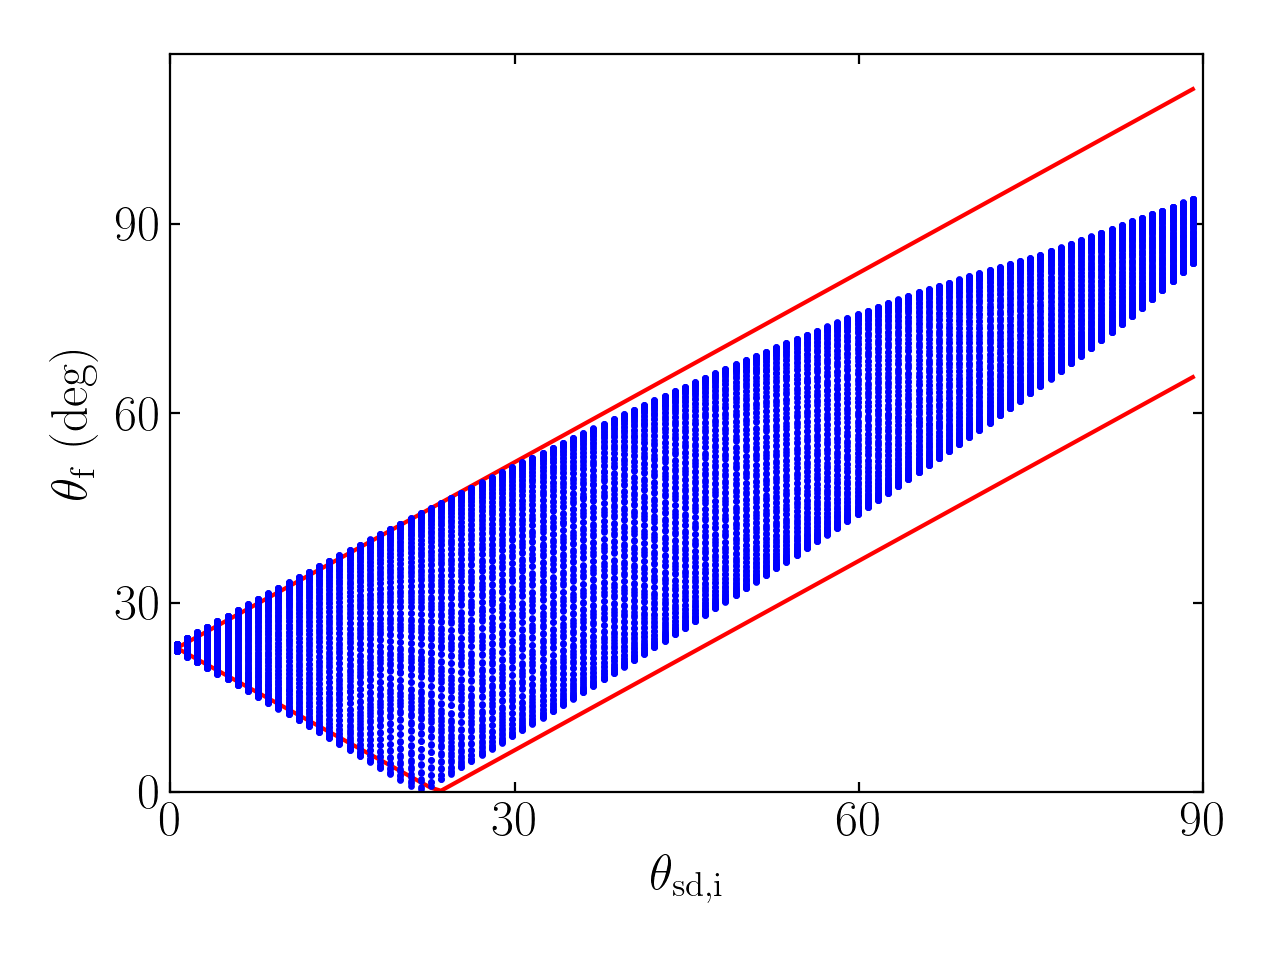
\includegraphics[width=\columnwidth]{../initial/2_toy2/3_ensemble_05_05.png}
    \caption{$\theta_{ f}\p{\theta_{sd, i}}$ at $\epsilon = 0.3$, firmly in
    the non-adiabatic regime. Note the clear double-valuedeness has disappeared,
    as have distinct dynamical histories. The red dotted line presents the
    analytical prediction given by
    \autoref{eq:nonad_q_f_dist}.}\label{fig:nonad_3_ensemeble}
\end{figure}

\subsection{Transition from Adiabaticity}

The agreement of \autoref{eq:nonad_q_f} at fixed $I$ for varying $\epsilon$ is
shown in \autoref{fig:nonad_3_scan}. Note that $\epsilon \to 0$ recovers the
adiabatic regime.
\begin{figure}
    \centering
    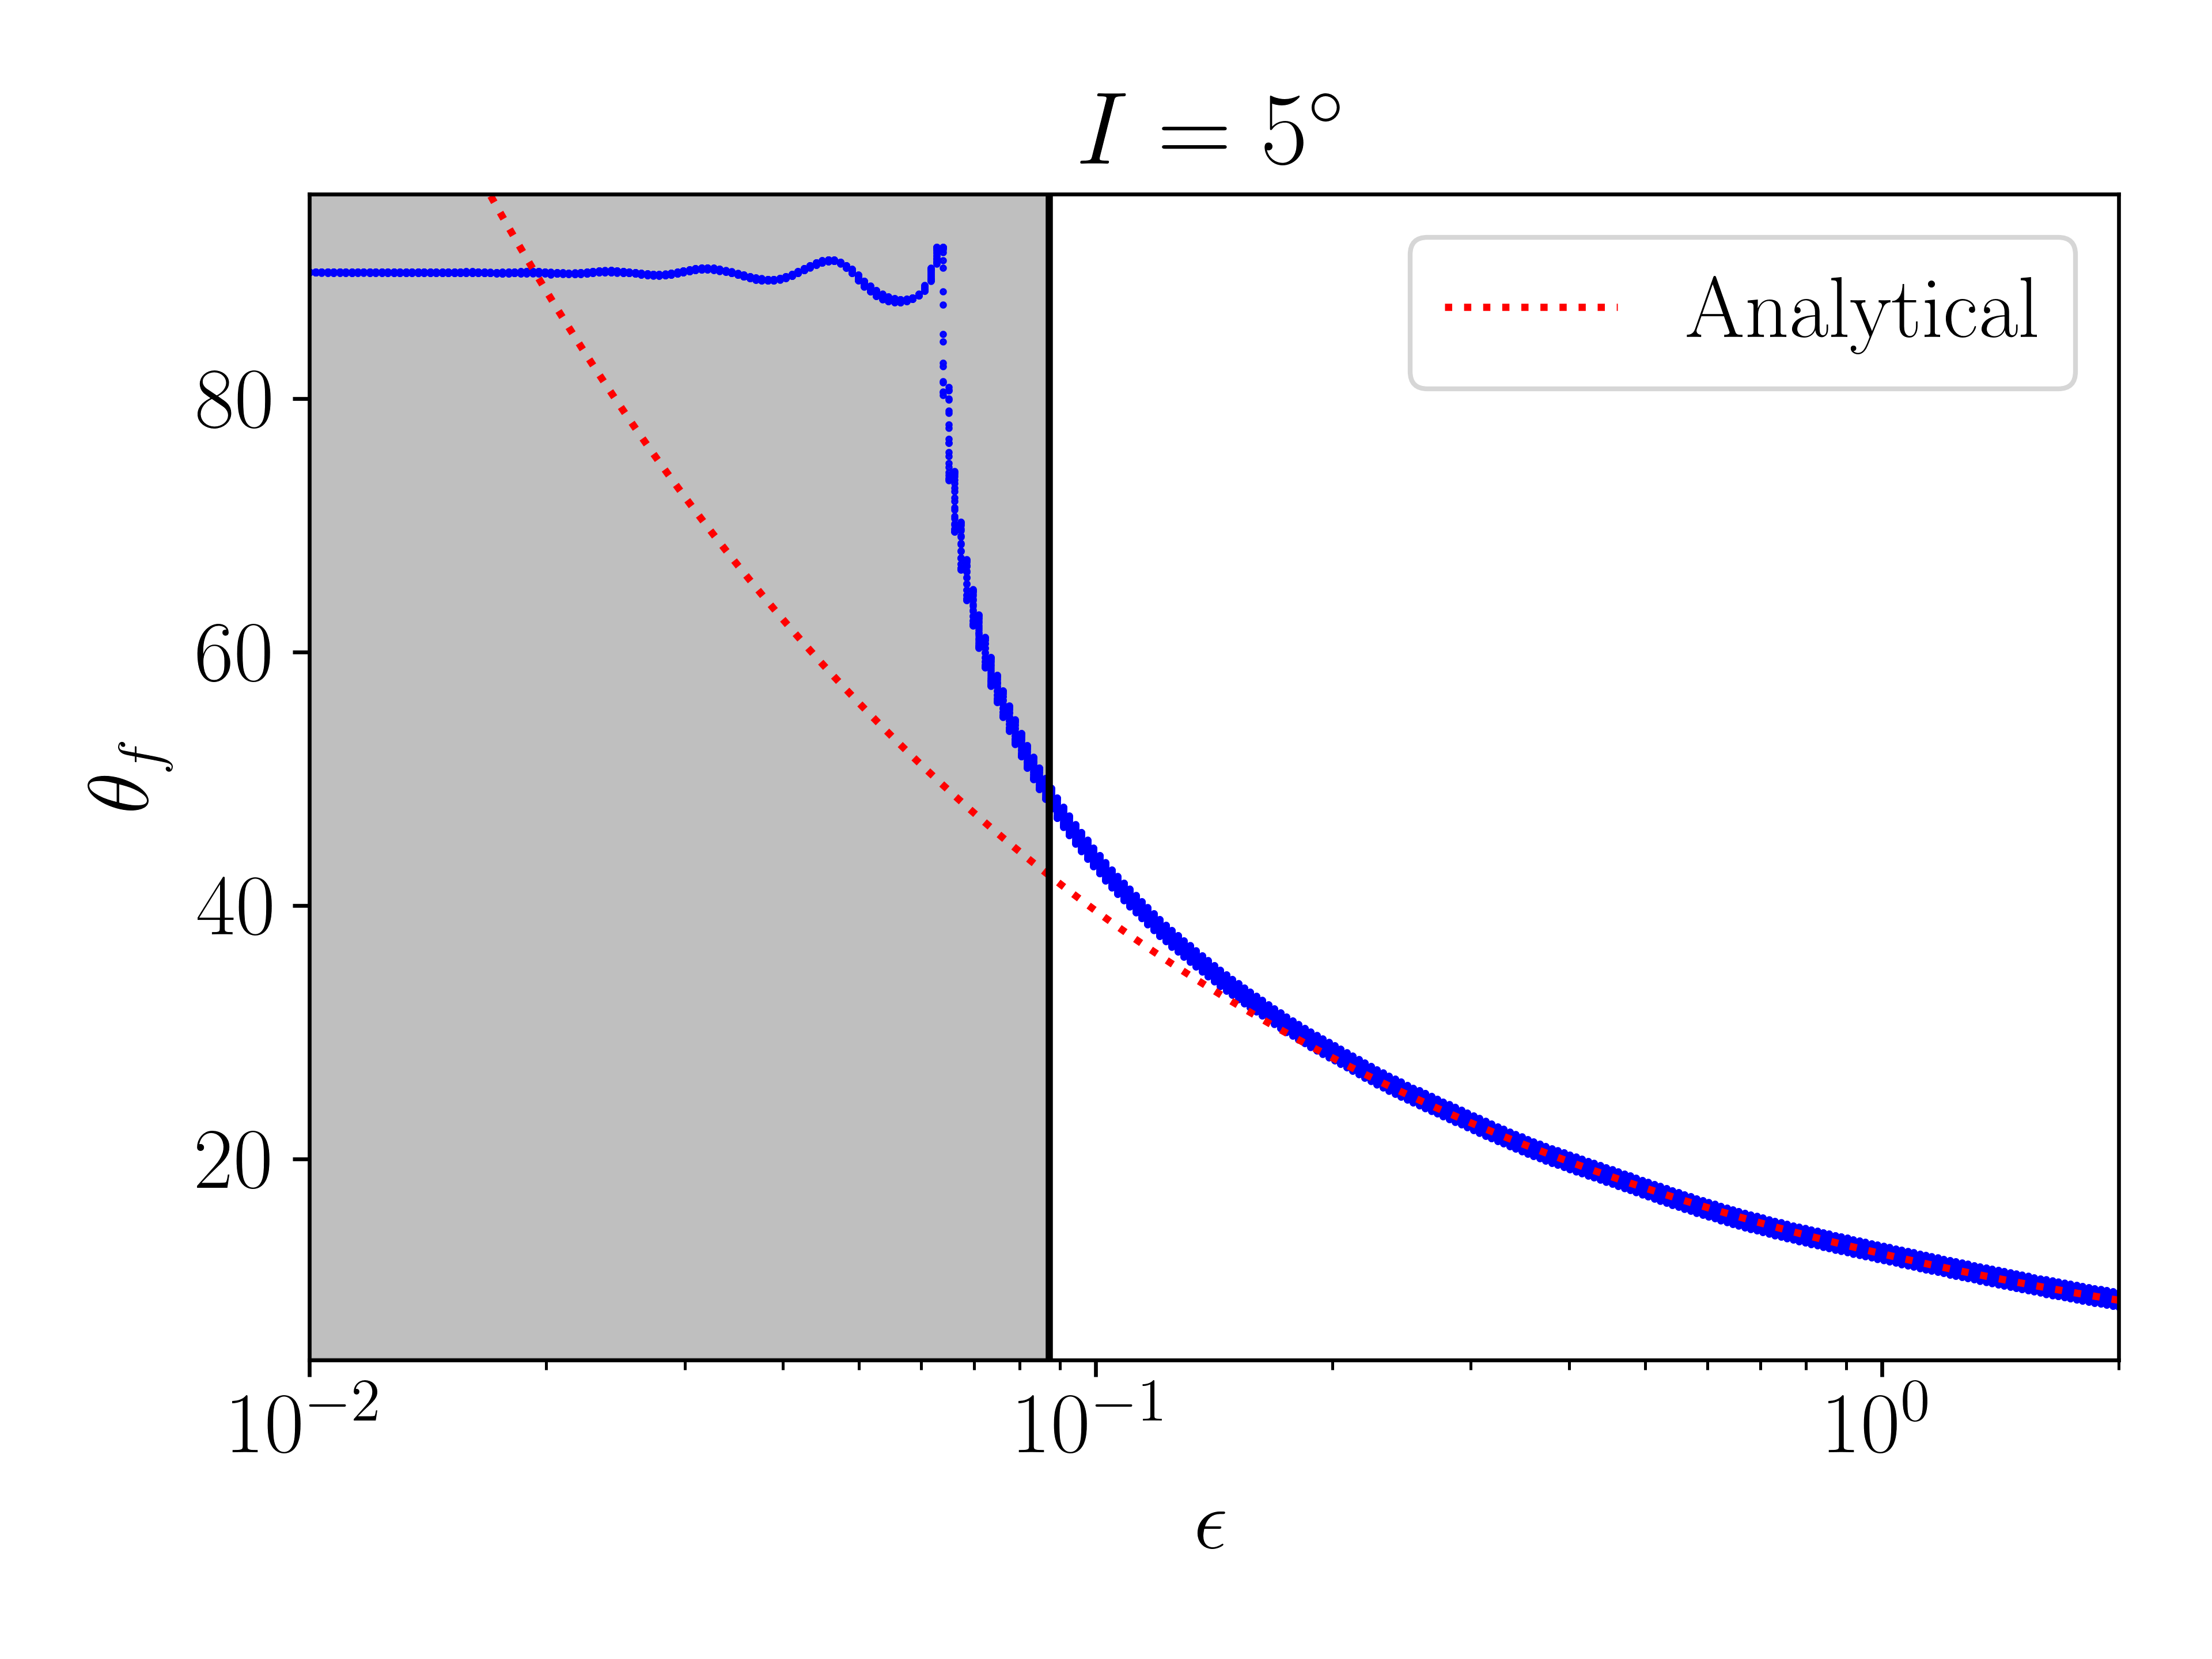
\includegraphics[width=\columnwidth]{../initial/2_toy2/3scan.png}
    \caption{Plot of $\theta_{ f}\p{\theta_{sd, i} = 0}$ as a function of
    $\epsilon$, where $I = 5^\circ$. Overplotted in the red line is
    \autoref{eq:nonad_q_f}, which is in good agreement for $\epsilon \gtrsim
    0.1$ the non-adiabatic regime, while $\theta_{ f} \approx 90^\circ$ in
    the adiabatic regime.}\label{fig:nonad_3_scan}
\end{figure}

An example of an intermediate value $\epsilon = 10^{-2}$ between
\autoref{fig:ad_ensemble} and \autoref{fig:nonad_3_ensemeble} is shown in
\begin{figure}
    \centering
    \includegraphics[width=\columnwidth]{../initial/2_toy2/3_ensemble_05_20.png}
    \caption{Intermediate $\epsilon$ used in between those of
    \autoref{fig:ad_ensemble} and \autoref{fig:nonad_3_ensemeble}. Noticeable
    ``freezing-in'' of the obliquity variations over libration cycles is still
    visible, but the shapes of the adiabatic dynamical trajectories are
    beginning to appear.}\label{fig:nonad_3_ensemble_20}
\end{figure}

TODO compare to \autoref{eq:ad_constr}.

\bibliographystyle{mnras}
\bibliography{Su_sep_cross}

% \clearpage
% \onecolumn
\appendix

\section{Dynamical Histories}\label{s:app_histories}

\begin{itemize}
    \item $A_2 \to A_1$ --- \autoref{fig:ad_21}.
    \item $A_2 \to A_3$ --- \autoref{fig:ad_23}.
    \item $A_3 \to A_1$ --- \autoref{fig:ad_31}.
    \item $A_3 \to A_2 \to A_1$ --- \autoref{fig:ad_321}.
    \item $A_3 \to A_3$ --- Trivial case, the initial enclosed area is too large
        to ever experience a separatrix encounter.
\end{itemize}
\begin{figure}
    \centering
    \begin{subfigure}{\columnwidth}
        \centering
        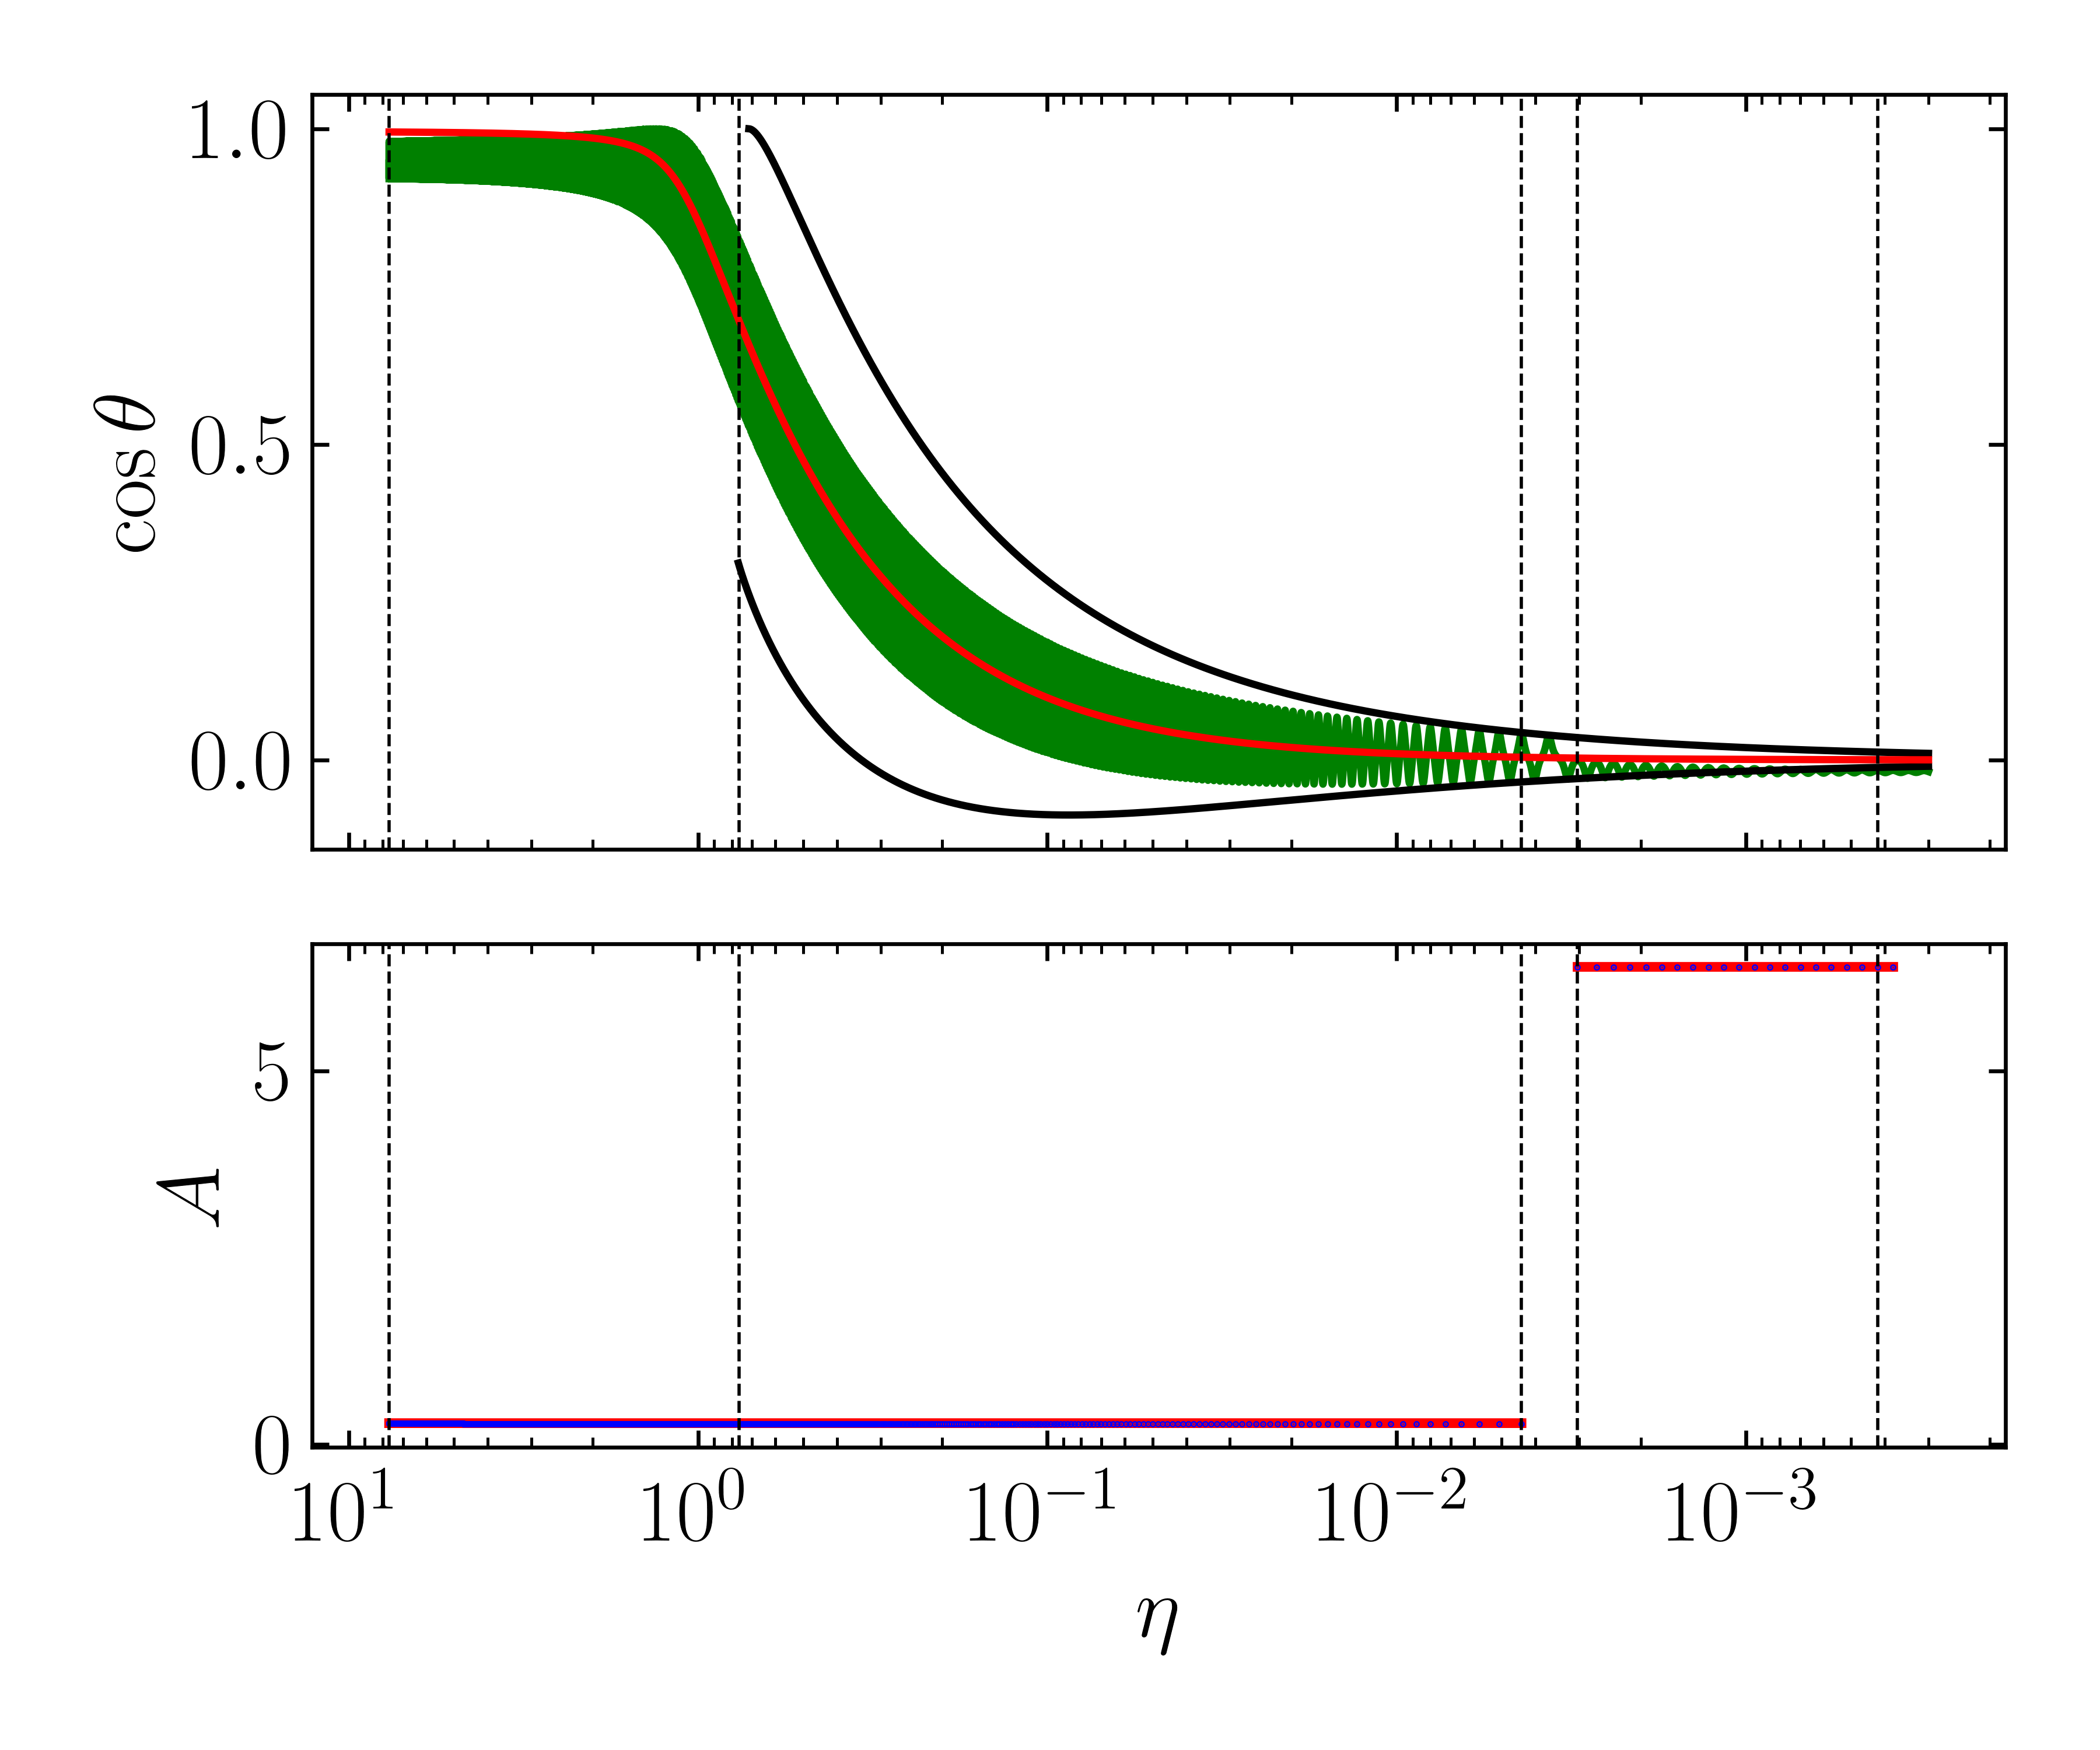
\includegraphics[width=\columnwidth]{../initial/2_toy2/3testo23.png}
    \end{subfigure}
    \begin{subfigure}{\columnwidth}
        \centering
        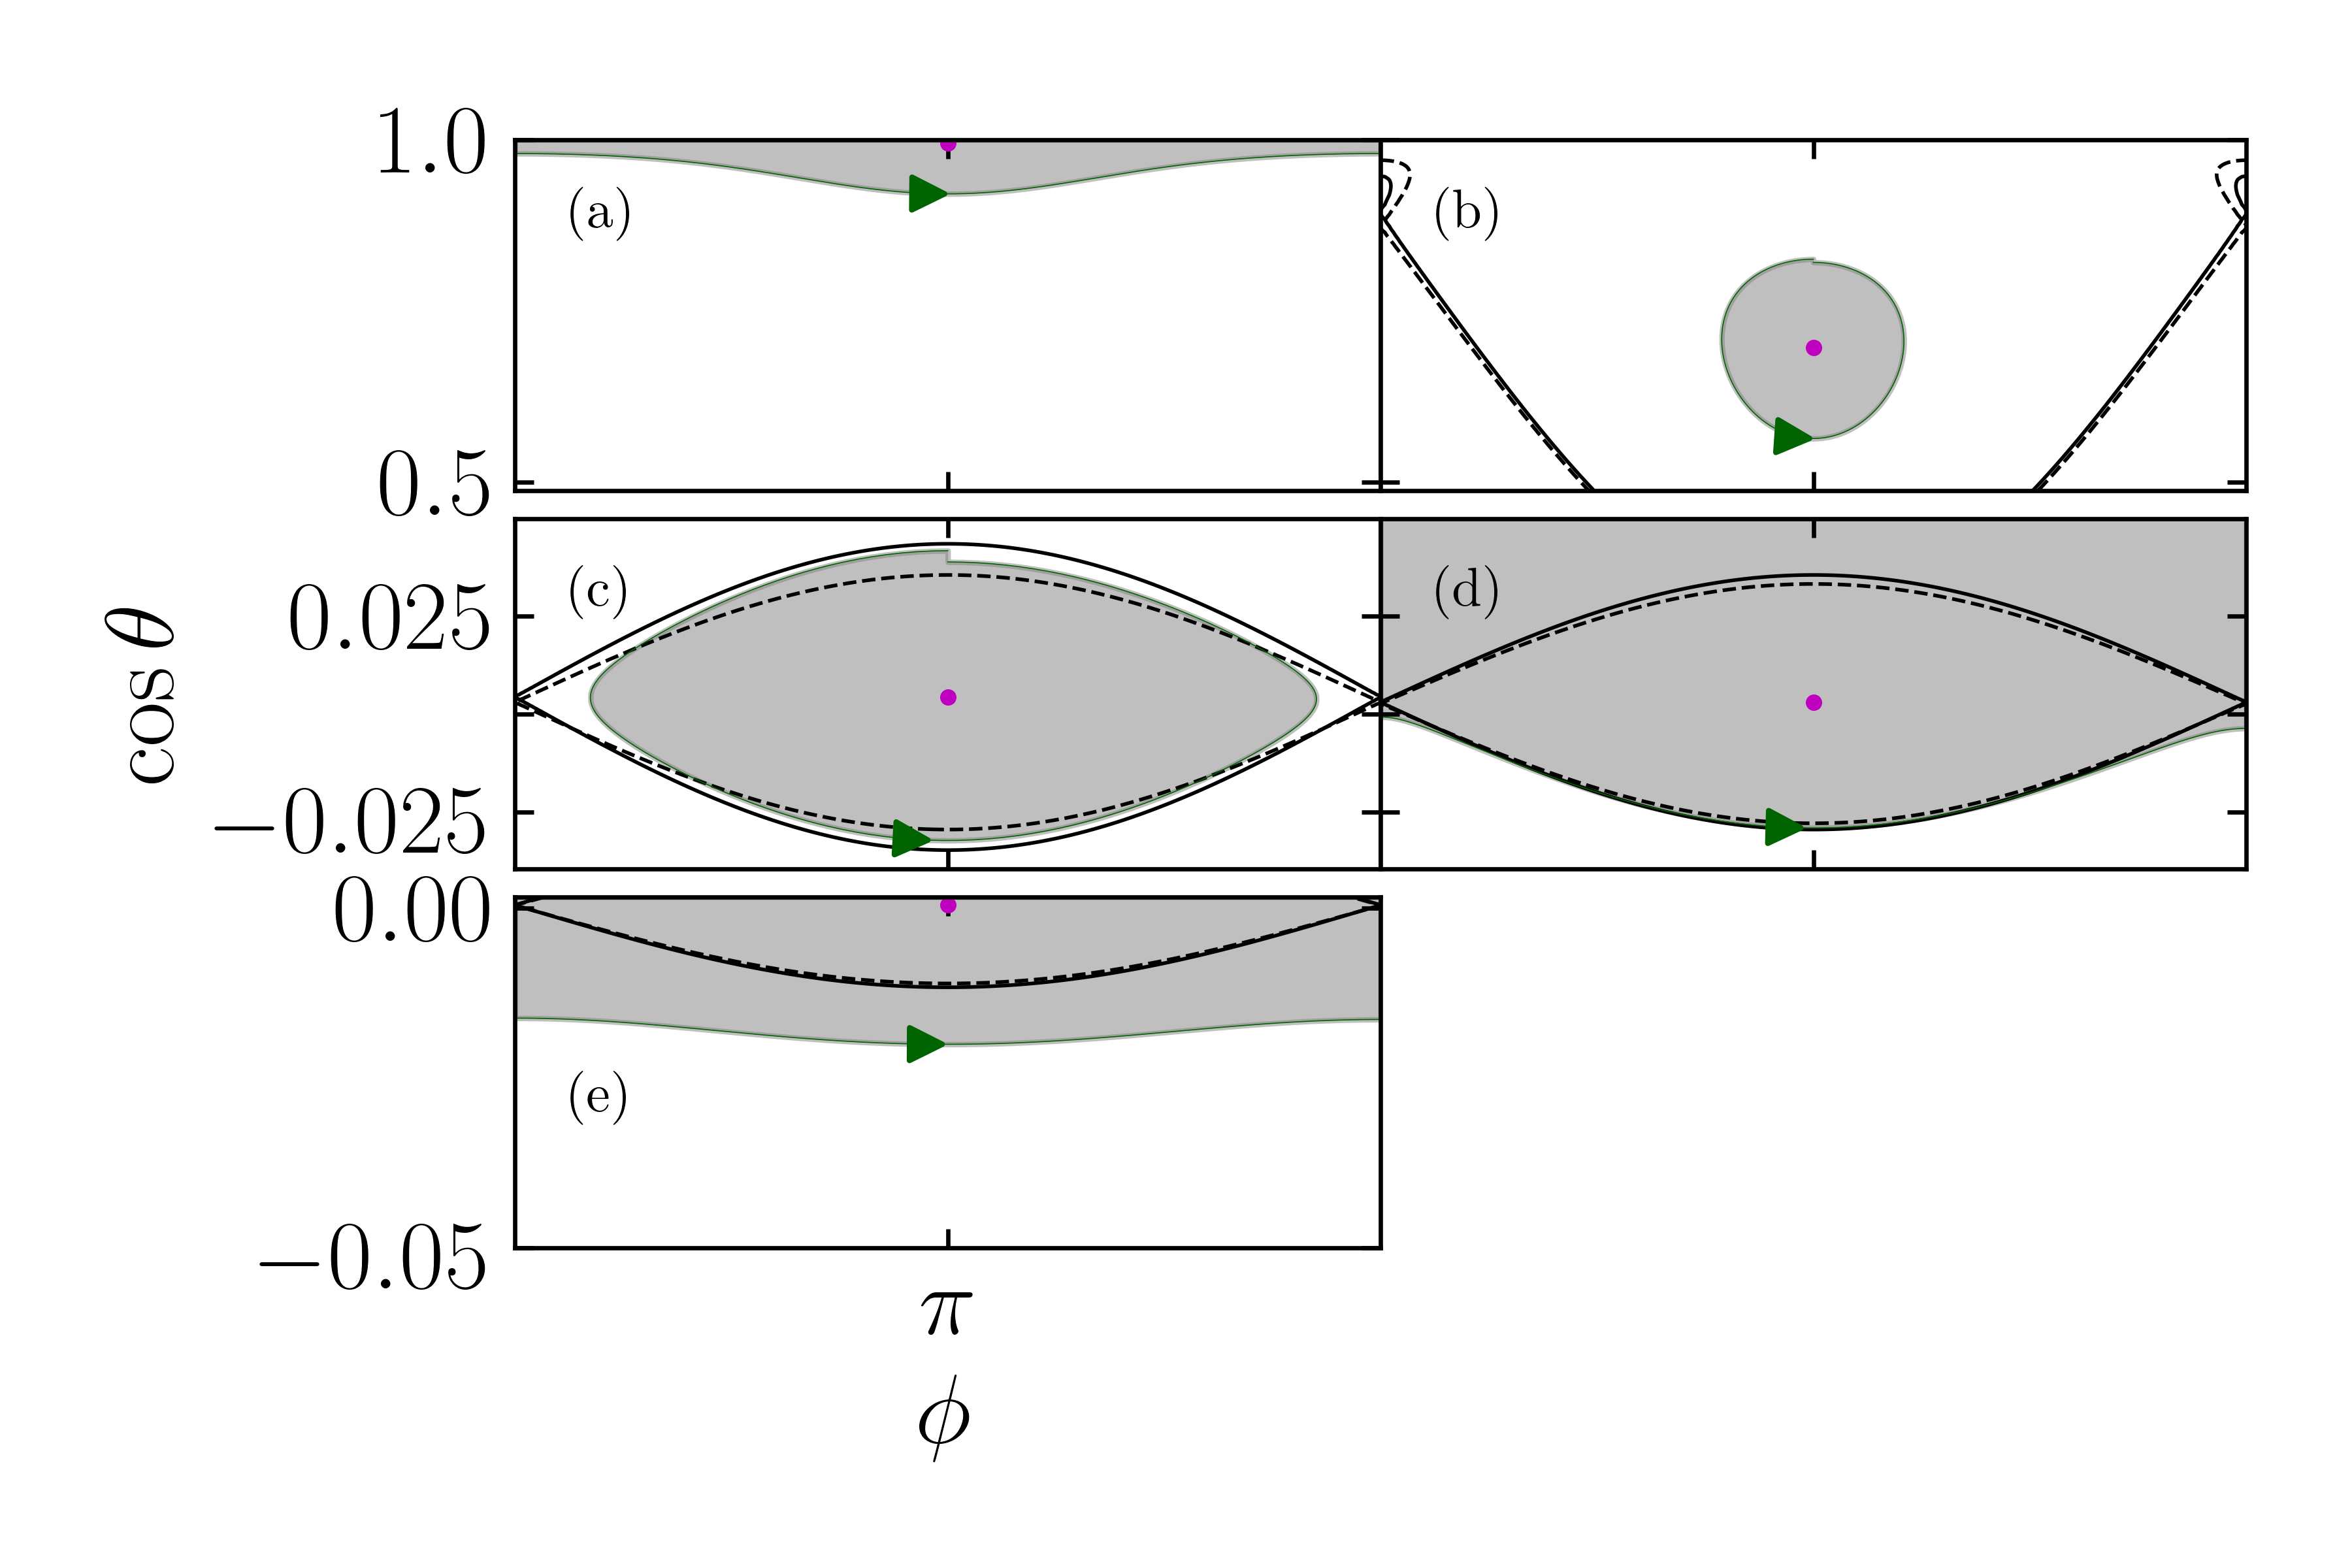
\includegraphics[width=\columnwidth]{../initial/2_toy2/3testo23_subplots.png}
    \end{subfigure}
    \caption{Same as \autoref{fig:ad_21} but for the $A_2 \to A_3$ history.
    }\label{fig:ad_23}
\end{figure}
\begin{figure}
    \centering
    \begin{subfigure}{\columnwidth}
        \centering
        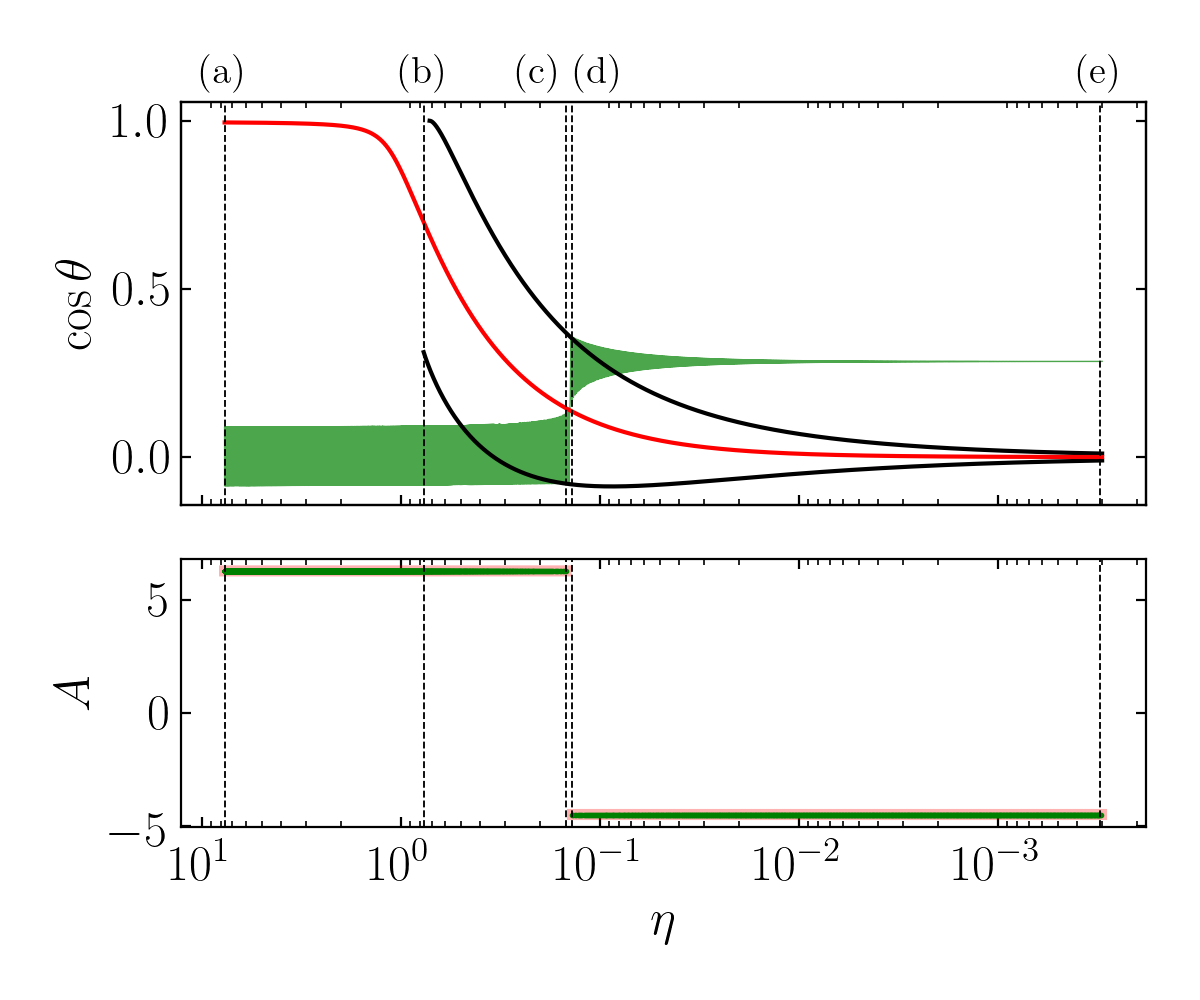
\includegraphics[width=\columnwidth]{../initial/2_toy2/3testo31.png}
    \end{subfigure}
    \begin{subfigure}{\columnwidth}
        \centering
        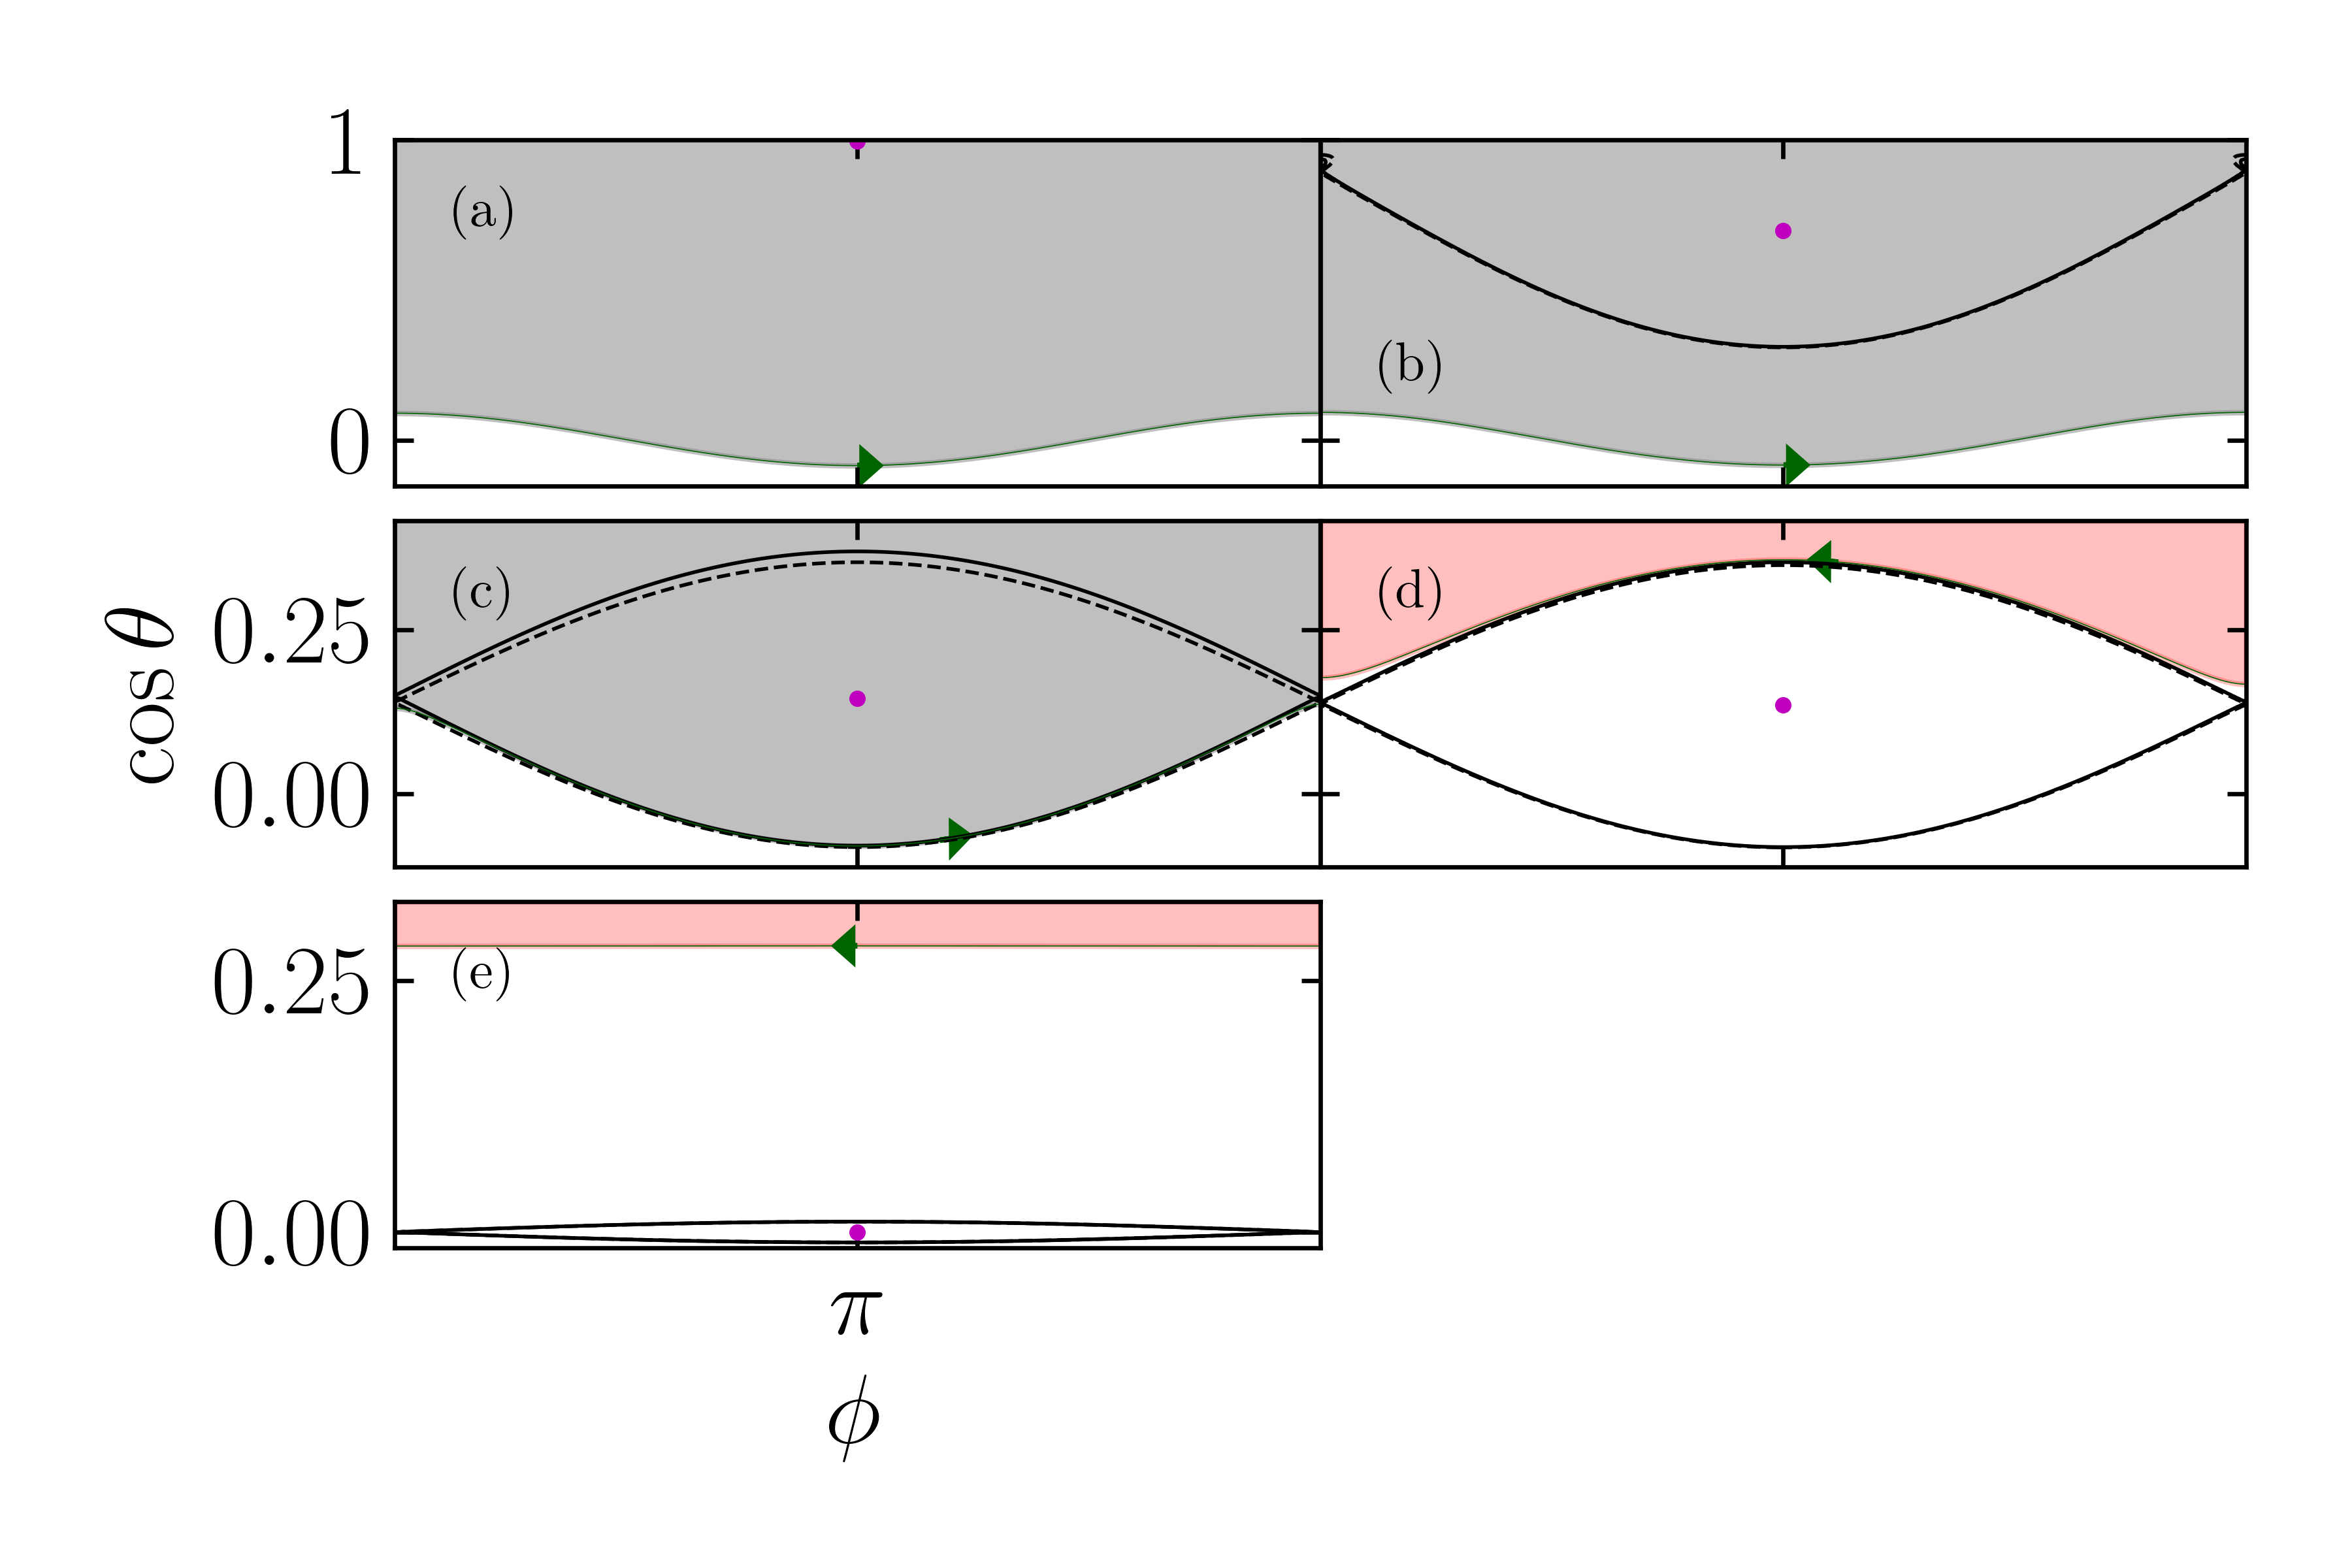
\includegraphics[width=\columnwidth]{../initial/2_toy2/3testo31_subplots.png}
    \end{subfigure}
    \caption{Same as \autoref{fig:ad_21} but for the $A_3 \to A_1$ history. TODO
    finish final areas plot.}\label{fig:ad_31}
\end{figure}
\begin{figure}
    \centering
    \begin{subfigure}{\columnwidth}
        \centering
        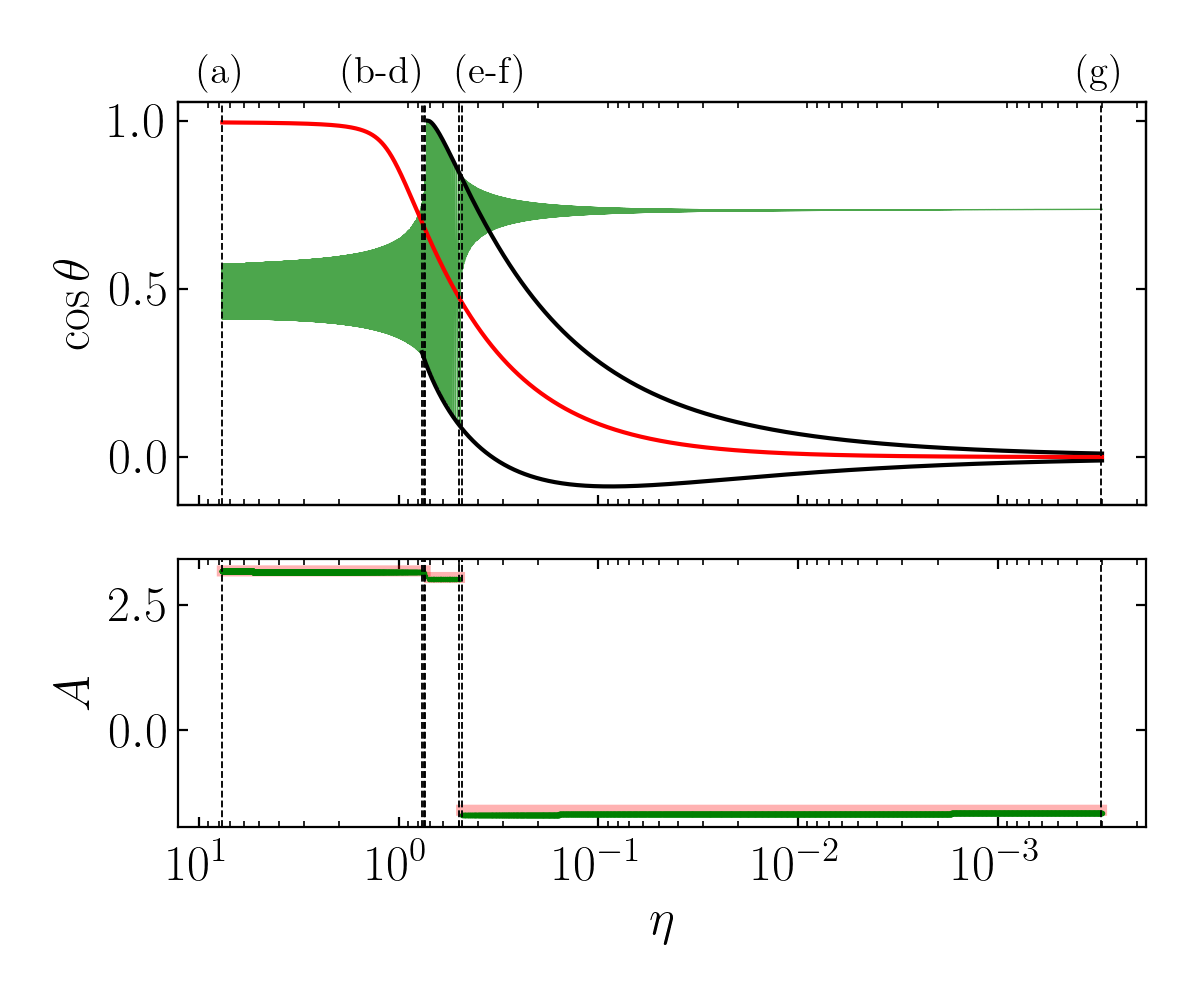
\includegraphics[width=\columnwidth]{../initial/2_toy2/3testo321.png}
    \end{subfigure}
    \begin{subfigure}{\columnwidth}
        \centering
        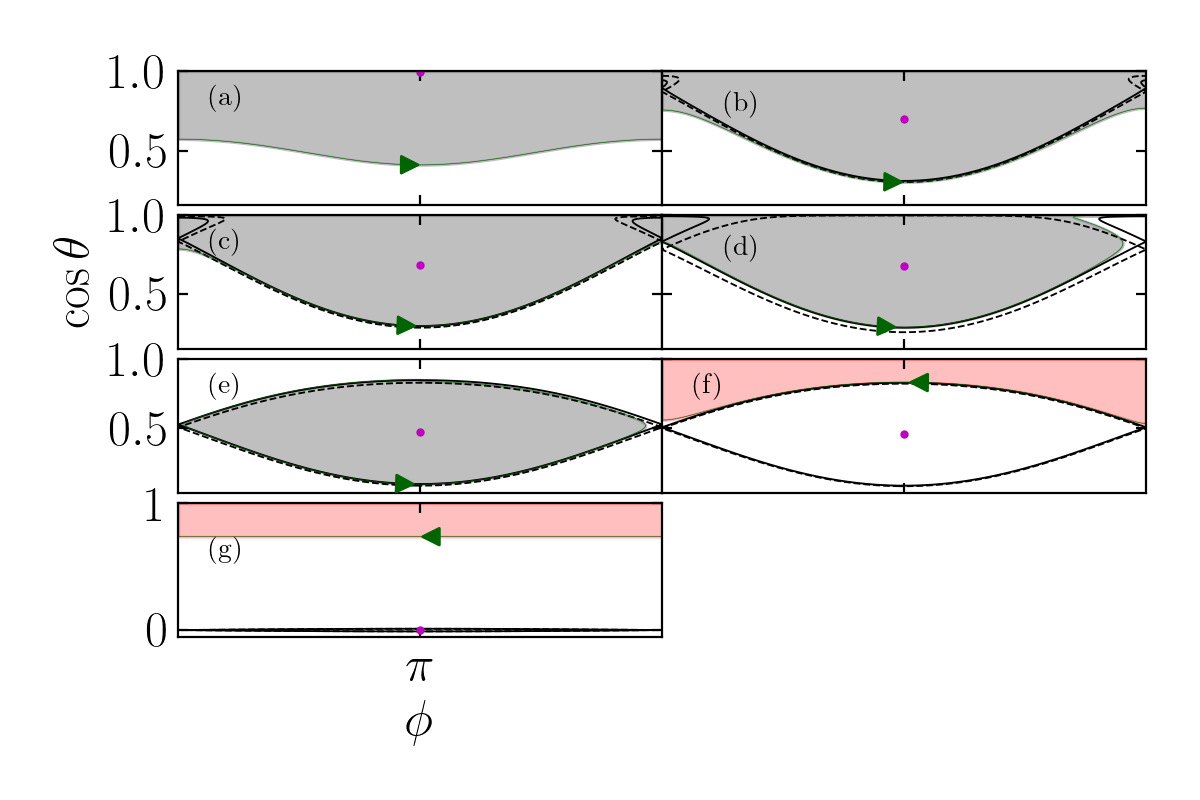
\includegraphics[width=\columnwidth]{../initial/2_toy2/3testo321_subplots.png}
    \end{subfigure}
    \caption{Same as \autoref{fig:ad_21} but for the $A_3 \to A_2 \to A_1$
    history. The second snapshot, instead of depicting the appearance of the
    separatrix, captures the first of the two separatrix crossings. TODO finish
    final areas plot.}\label{fig:ad_321}
\end{figure}

\section{Variation with $I$}

Plots of \autoref{fig:ad_ensemble} but for $I = 10^\circ, I=20^\circ$.

\section{Calculation of Transition Probabilities}\label{ss:app_transition}

Semi-analytic calculation probabilities, including naive line.

\label{lastpage} % chktex 24
\end{document}
